
%#############################################################
%MAIN file for  project
%#############################################################
\documentclass[12pt]{report}
%############################################################
%###### Package 'name' 
%###### This package contains ...
%###### Author  : Nicolas LE GUERROUE
%###### Contact : nicolasleguerroue@gmail.com
%############################################################
\RequirePackage{lmodern}
\RequirePackage[T1]{fontenc}
\RequirePackage[utf8]{inputenc}     %UTF-8 encoding
\RequirePackage[many]{tcolorbox}
%1 : txt color
%2 : bg color 
%3 : text
\newtcbox{\badge}[3][red]{
  on line, 
  arc=2pt,
  colback=#3,
  colframe=#3,
  fontupper=\color{#2},
  boxrule=1pt, 
  boxsep=0pt,
  left=6pt,
  right=6pt,
  top=2pt,
  bottom=2pt
}

%################################################################%############################################################
%###### Package 'Chapter_1' 
%###### This package contains first model of chapter
%###### Author  : Nicolas LE GUERROUE
%###### Contact : nicolasleguerroue@gmail.com
%############################################################
% \RequirePackage[explicit]{titlesec} 


% \titleformat{\chapter}
%   {\gdef\chapterlabel{}
%    \normalfont\sffamily\Huge\bfseries\scshape}
%   {\gdef\chapterlabel{\thechapter)\ }}{0pt}
%   {\begin{tikzpicture}[remember picture,overlay]
%     \node[yshift=-2cm] at (current page.north west)
%       {\begin{tikzpicture}[remember picture, overlay]
%         \draw[fill=MediumBlue] (0,0) rectangle
%           (\paperwidth,2cm);
%         \node[anchor=east,xshift=.9\paperwidth,rectangle,
%               rounded corners=20pt,inner sep=11pt,
%               fill=white]
%               {\color{black}#1};%\chapterlabel
%           \node[anchor=west,yshift=1cm,xshift=2cm,inner sep=11pt,
%               fill=MediumBlue]
%               {\color{white}{\large Synthèse Latex}};%\chapterlabel
%        \end{tikzpicture}
%       };
%    \end{tikzpicture}
%   }
%   \titlespacing*{\chapter}{0pt}{50pt}{-60pt}%############################################################
%###### Package 'Color' 
%###### This package contains some colors
%###### Author  : Nicolas LE GUERROUE
%###### Contact : nicolasleguerroue@gmail.com
%############################################################
\RequirePackage{color}              %colors
%################################################################
\definecolor{pathColor}{rgb}{0.858, 0.188, 0.478}
\definecolor{fileColor}{rgb}{0.858, 0.188, 0.478}
\definecolor{water}{rgb}{0.858, 0.188, 0.478}
\definecolor{LightBlue}{RGB}{66, 163, 251}
\definecolor{DarkBlue}{RGB}{36, 100, 176}
\definecolor{LightGray}{gray}{.94}
\definecolor{DarkGray}{gray}{.172}
\definecolor{Orange}{RGB}{229, 133, 3}
\definecolor{MediumBlue}{RGB}{38, 119, 193}


\newcommand{\colors}[2]{
{\color{#1}{#2}}
}%############################################################
%###### Package 'Check' 
%###### This package contains soem tools to check data
%###### Author  : Nicolas LE GUERROUE
%###### Contact : nicolasleguerroue@gmail.com
%############################################################
%################################################################

  \makeatletter%
  \@ifpackageloaded{babel}
    {\typeout{>>> Utils : Babel package is loaded}}%
    {\typeout{>>> Utils : Babel package is not loaded}}%
  \makeatother%%############################################################
%###### Package 'Electronic' 
%###### This package contains some tools to generate electornic circuits
%###### Author  : Nicolas LE GUERROUE
%###### Contact : nicolasleguerroue@gmail.com
%############################################################

\RequirePackage{tikz-timing}

\RequirePackage{graphics} %include figures
\RequirePackage{graphicx} %include figures
\RequirePackage{pgf,tikz}
\RequirePackage{circuitikz}
\usetikzlibrary{babel}  %allow to use tikz library with babel

\RequirePackage{ifthen}    %use if then 
 

%############################ Settings ##############################
\tikzset{%
    timing/table/axis/.style={->,>=latex},
    timing/table/axis ticks/.style={},   
}

%Direction of some device such as resistor, led...
%1.5 is the minimum length of device according my runs
\newcommand{\Up}{0,1.5}
\newcommand{\Down}{0,-1.5}
\newcommand{\Right}{1.5,0}
\newcommand{\Left}{-1.5,0}


%###### Length of components
\newcommand{\bipolesLength}[1]{#1cm}     %begin default size
%Length update
\newcommand{\setBipolesLength}[1]{
    \renewcommand{\bipolesLength}{#1}
    \ctikzset{bipoles/length=\bipolesLength cm}
}%End \setBipolesLength

%############ Mirrors and inverting
\newcommand{\Mirror}{}
\newcommand{\Invert}{}

%Update
\newcommand{\setMirror}[1]{
    \renewcommand{\Mirror}{,mirror}
}%End \setMirror

\newcommand{\setNoMirror}[1]{
    \renewcommand{\Mirror}{}
}%End \setMirror

\newcommand{\setInvert}[1]{
    \renewcommand{\Invert}{,Invert}
}%End \setInvert

\newcommand{\setNoInvert}[1]{
    \renewcommand{\Invert}{}
}%End \setInvert


%############## Rotate ###########
\newcommand{\rotate}{0}

%Update
\newcommand{\setRotate}[1]{
    \renewcommand{\rotate}{#1}
}%End \setRotate


%####################### Colors
%default colors of border colors and background colors
\newcommand{\deviceBorderColor}{black}
\newcommand{\deviceBackgroundColor}{white}

%Update
\newcommand{\setDeviceBorderColor}[1]{
    \renewcommand{\deviceBorderColor}{#1}
    \renewcommand{\deviceBackgroundColor}{white} %reset bg color
}%End \setDeviceBorderColor

\newcommand{\setDeviceBackgroundColor}[1]{
    \renewcommand{\deviceBorderColor}{black} %reset bg color
    \renewcommand{\deviceBackgroundColor}{#1}
}%\setDeviceBackgroundColor

%Reset
\newcommand{\resetColors}{
    \renewcommand{\deviceBorderColor}{black} %reset border color
    \renewcommand{\deviceBackgroundColor}{white} %reset bg color
}
%####################################################################
%############## draw device #########################################

%rotation
%color
%anchor

%\ifthenelse{\equal{#1}{0}}{A.}{no A.}
%Init

\begin{comment}
    @begin
    @command \addLogicGate
    @des 
    Cette commande permet de dessiner une porte logique à double entrée. Pour dessinder une porte inverseuse, utiliser la commande \addNotGate
    @sed
    @input Coordonnées de la porte en (x,y) sans parenthèse
    @input Référence de la porte pour s'accrocher aux entrées et sorties
    @input Type de la porte [nand, nor, or, and, or, xor]
    @input Label de sortie (laisser vide si absence de label souhaité)
    @input Label de l'entrée 1 (laisser vide si absence de label souhaité)
    @input Label de l'entrée 2 (laisser vide si absence de label souhaité)
    @input Nom de la porte [NOR1, AND1...]
    @begin_example 
    \addLogicGate{5,5}{logicgate}{nand}{S}{A}{B}{L1}
    @end_example
    @end
    \end{comment}

\newcommand{\addLogicGate}[7] {
    %\Colors
    \raiseMessage{Adding logic gate device [type=#3]}
    \ifthenelse{\equal{\deviceBorderColor}  {black}}
    {\draw (#1)         node (#2) [rotate=\rotate,xshift=0cm,fill=\deviceBackgroundColor,#3 port] {#7}}%if equal to black
    {\draw (#1)         node (#2) [rotate=\rotate,xshift=0cm,color=\deviceBorderColor,#3 port] {#7}}

    (#2.out)  node      [anchor=south west, yshift=-0.3cm] {#4}
    (#2.in 1) node (A1)     [anchor=east,xshift=0cm,yshift=+0.3cm]       {#5}
    (#2.in 2) node (B1)     [anchor=east,xshift=0cm,yshift=+0.3cm]       {#6};
}


\newenvironment{schema}[1]
{
    \begin{center}
        \makeatletter
        \def\@captype{figure}
        \makeatother
        \newcommand{\TitleSchema}{#1}%use var to print title 
        %\shorthandoff{:;!?} %Compulsory if frenchb package is used (from babel)
        \raiseMessage{Creating new schema ['#1']}
        \begin{tikzpicture}
            %\setGraphic %command to display with frenchb babel
    }
    { 
        \end{tikzpicture}
   % \caption{\TitleSchema}
    \end{center}
}


\newenvironment{numeric}[1]
{
\begin{center}
    \makeatletter
    \def\@captype{figure}
    \makeatother
    \newcommand{\TitleNumeric}{#1}%use var to print title 
    \raiseMessage{Creating new chronogram ['#1']}
\begin{tikztimingtable}
}
{
\end{tikztimingtable}%
\caption{\TitleNumeric}
\end{center}
}


%cood
%name device
%type (npn, pnp)
%B
%C
%E
\newcommand{\addTransistor}[6] {

    \raiseMessage{Adding transistor device [type=#3]}
    \ifthenelse{\equal{\deviceBorderColor}  {black}}
    {\draw (#1)         node (#2) [xshift=0cm,fill=\deviceBackgroundColor,#3] {}}%if equal to black
    {\draw (#1)         node (#2) [xshift=0cm,color=\deviceBorderColor,#3] {}}

    (#2.B)  node      [anchor=south west, xshift=0cm, yshift=0cm] {#4} 
    (#2.C) node (A1)     [anchor=north,xshift=0.3cm,yshift=+0.1cm]       {#5}
    (#2.E) node (B1)     [anchor=south,xshift=0.3cm,yshift=0.1cm]       {#6};
}
%node 1
%node 2
%wire type
\newcommand{\addWire}[3] {
    \draw (#1) #3 (#2);
}%end addWire

\newcommand{\orthogonalWireA}{-|}
\newcommand{\orthogonalWireB}{|-}
\newcommand{\directWire}{--}

%coord
%label
%value
\newcommand{\addNode}[3] {
    \node (#2) at (#1) {#3};
}%end addWire


%posiition (x,y)
%color
%width in pt
\newcommand{\addPoint}[3] {
    \filldraw [#2] (#1) circle (#3pt);
}%end addWire

%posiition (x,y)
%name
%value
\newcommand{\addPower}[3] {
    \raiseMessage{Adding power device [name=#2, value=#3]}
    \draw (#1) node (#2) [vcc] {#3};
}%end addPower

%posiition (x,y)
%name
%value
\newcommand{\addGround}[3] {
    \draw (#1) node (#2) [ground] {#3};
}%end addGround

%posiition depart(x,y)
%orientation de départ
%position arrivée
\newcommand{\addResistor}[4] {
    \raiseMessage{Adding resistor device}
    \draw (#1) to[R,l=$R$] +(#2) #4 (#3);
}%end addResistor

%posiition depart(x,y)
%orientation de départ
%position arrivée
%type de liaison
%nom de la led
\newcommand{\addLed}[5] {
    \raiseMessage{Adding LED device [name=#5]}
    \ifthenelse{\equal{\deviceBorderColor}  {black}}
    {\draw (#1) to[leD,l_=#5,fill=\deviceBackgroundColor] +(#2) #4 (#3);}
    {\draw (#1) to[leD,l_=#5,color=\deviceBorderColor] +(#2) #4 (#3);}

    % {\draw (#1)         node (#2) [xshift=0cm,fill=\deviceBackgroundColor,#3] {}}%if equal to black
    % {\draw (#1)         node (#2) [xshift=0cm,color=\deviceBorderColor,#3] {}}

    %\draw (#1) to[leD,l_=#5] +(#2) #4 (#3);
}%end addResistor%############################################################
%###### Package 'Font' 
%###### This package contains some tools to set fonts
%###### Author  : Nicolas LE GUERROUE
%###### Contact : nicolasleguerroue@gmail.com
%############################################################
\RequirePackage{fontawesome}

   %############################################################
%###### Package 'Glossaries' 
%###### This package contains some tools to set glossaries
%###### Author  : Nicolas LE GUERROUE
%###### Contact : nicolasleguerroue@gmail.com
%############################################################
\RequirePackage[xindy, acronym, nomain, toc]{glossaries}
%################################################################
\makeglossaries

\renewcommand{\glossary}[1]{%
\gls{#1}
}%############################################################
%###### Package 'Graphics' 
%###### This package contains some tools to create graphics 2D or 3D
%###### Author  : Nicolas LE GUERROUE
%###### Contact : nicolasleguerroue@gmail.com
%############################################################
%\ProvidesPackage{Utils}[2013/01/13 Utils Package]
%############################################################
\RequirePackage[T1]{fontenc}
\RequirePackage[utf8]{inputenc}     %UTF-8 encoding
\RequirePackage{csvsimple} 
\RequirePackage{tikz,pgfplots,pgf}  
\RequirePackage{version}            %use commented code

\RequirePackage{graphics} %include figures
\RequirePackage{graphicx} %include figures
\RequirePackage{caption}
\RequirePackage{subcaption} %Add
\RequirePackage{version}            %use commented code
\pgfplotsset{compat=1.7}
%###### Checking if babel is loaded
\makeatletter
\@ifpackageloaded{babel}
{% if the package was loaded
\newcommand{\setGraphic}{\shorthandoff{:;!?}} %Compulsory if frenchb package is used (from babel)
\frenchbsetup{StandardLists=true} %to include if using \RequirePackage[french]{babel} -> rounded list
}
{%else:
\newcommand{\setGraphic}{} %Compulsory if frenchb package is used (from babel)
}
\makeatother
%############################################################
%### WARNING : USE \shorthandoff{:;!?} before \begin{tikzpicture} 
%### environment
%############################################################
\begin{comment}
@begin
@env graphics
@des 
Cet environnement permet de tracer des courbes en 2D à partir de points, d'équations ou de fichier CSV
@sed
@input Largeur du graphique ]0;1] 
@input Hauteur du graphique ]0;1+] 
@input Valeur minimale en abscisse 
@input Valeur maximale en abscisse
@input Valeur minimale en ordonnée 
@input Valeur maximale en ordonnée
@input Légende de l'axe des abscisse
@input Légende de l'axe des ordonnées
@input Titre du graphique
@begin_example 
\begin{graphics}{0.8}{0.5}{0}{100}{-10}{10}{ve}{vs}{Titre}
\addPointsFromCSV{raw.csv}
\end{graphics}
@end_example
@end
\end{comment}

\newenvironment{graphicFigure}[9]
{
    \raiseMessage{Creating new graphic figure [title='#9']}
    \begin{center}
        \makeatletter
        \def\@captype{figure}
        \makeatother

        \newcommand{\TitleGraphic}{#9}%use var to print title 
        \begin{tikzpicture}
        \setGraphic %command to display with frenchb babel
    %\shorthandoff{:;!?} %Compulsory if frenchb package is used (from babel)
    \begin{axis}[width=#1\linewidth,height=#2\linewidth,xmin=#3,xmax=#4,  ymin=#5, ymax=#6, scale only axis,xlabel=#7,ylabel=#8] %grid=both
    }
    { 
    \end{axis}
        \end{tikzpicture}
        \captionof{figure}{\TitleGraphic}
    \end{center}
}


\newenvironment{graphic}[9]
{
    \raiseMessage{Creating new graphic [title='#9']}
    \newcommand{\TitleGraphic}{#9}%use var to print title 
        \begin{tikzpicture}
        \setGraphic %command to display with frenchb babel
    \begin{axis}[width=#1\linewidth,height=#2\linewidth,xmin=#3,xmax=#4,  ymin=#5, ymax=#6, scale only axis,xlabel=#7,ylabel=#8, title=#9] %grid=both
    }
    { 
    \end{axis}
        \end{tikzpicture}

}
    
%############################################################
\begin{comment}
@begin
@command plot
@des 
Cette commande permet de tracer des surfaces 3D
@sed
@input Iitre du graphique
@input Equation à deux variables (x et y)
@begin_example 
\plot{Titre}{x*x+y*5}
@end_example
@end
\end{comment}   
    
\newcommand{\plot}[2]{
    \raiseMessage{Creating new plot [title='#1']}
\begin{tikzpicture}
\setGraphic %command to display with frenchb babel
 \begin{axis}[title={#1}, xlabel=x, ylabel=y]
 \addplot3[surf,domain=0:360,samples=50]
 {#2};
 \end{axis}
 \end{tikzpicture}
 }
    
%############################################################
\begin{comment}
@begin
@command addPoints
@des 
Cette commande permet de tracer une courbe en passant une liste de coordonnées de points : (x1,y1)(x2,y2)(...)
Il faut que cette commande soit utilisées dans l'environnement \textbf{graphics}.
@sed
@input Couleur de la courbe
@input Liste des coordonnées des points. Chaque point est entre parenthèse et les coordonnées sont séparées par une virgule
@begin_example 
\addPoints{red}{(0,0)(5,0)(5,5)(10,5)(10,0)}
@end_example
@end
\end{comment}   

\newcommand{\addPoints}[2]{
    \addplot+[thick,mark=none, color=#1] coordinates{#2};
}

%############################################################
\begin{comment}
@begin
@command addTrace
@des 
Cette commande permet de tracer une courbe en passant une équation en fonction de x
Il faut que cette commande soit utilisées dans l'environnement \textbf{graphics}.
@sed
@input Couleur de la courbe
@input Début du domaine de définition
@input Fin du domaine de définition
@input Équation à tracer
@begin_example 
\addTrace{blue}{4}{8}{8x^2}
@end_example
@end
\end{comment}

\newcommand{\addTrace}[4]{
    \addplot [#1, domain=#2:#3, samples=400] {#4};
}

%############################################################
\begin{comment}
@begin
@command addPointsFromCSV
@des 
Cette commande permet de tracer une courbe en passant un fichier de données CSV (ou format TXT)
Il faut que cette commande soit utilisées dans l'environnement \textbf{graphics}.
@sed
@input Couleur de la courbe
@input délimitateur des données (comma=virgule, semicolon=point-vigule)
@input Fichier des données
@begin_example 
\addPointsFromCSV{blue}{semicolon}{raw.csv}
@end_example
@end
\end{comment}

\newcommand{\addPointsFromCSV}[3]{
    \IfFileExists{#3}{
    \addplot+[thick, mark=none, color=#1] table[mark=none,col sep=#2] {#3};
    \raiseMessage{File '#3' loaded !}
    }
    {\raiseError{[import failed]'#3' \stop}
    }
}

%############################################################
\begin{comment}
@begin
@command addLegend
@des 
Cette commande permet d'ajouter une légende au graphique
Il faut que cette commande soit utilisées dans l'environnement \textbf{graphics}.
@sed
@input Légendes de chaque courbe séparées par une virgule
@begin_example 
\addLegend{sig1, sig2, sig3}
@end_example
@end
\end{comment}

\newcommand{\addLegend}[1]{
    \legend{#1}
}

%############################################################%############################################################
%###### Package 'Layout' 
%###### This package contains some tools to set page layout or text
%###### Author  : Nicolas LE GUERROUE
%###### Contact : nicolasleguerroue@gmail.com
%############################################################
\RequirePackage{lmodern}
\RequirePackage[T1]{fontenc}
\RequirePackage[utf8]{inputenc}     %UTF-8 encoding
\RequirePackage{graphicx}           %Images
\RequirePackage{caption}            %légende
\RequirePackage{textcomp}           %special characters
\RequirePackage{fancyhdr}           %headers & footers
\RequirePackage{lastpage}           %page counter

\RequirePackage{float}              %image floating
\RequirePackage{wrapfig}
\RequirePackage{subcaption}         %Subcaption

\RequirePackage{geometry}

%############################################################

\begin{comment}
@begin
@command \setHeader
@des 
Cette commande permet de créer une page de garde minimaliste
@sed
@input Titre du document
@input Auteur(s) - Les retours à la ligne se font en utilisant la commande \\
@input La date
@begin_example 
\setHeader{Titre}{Auteur 1 \\ Auteur 2}{XX/XX/XXXX}
@end_example
@end
\end{comment}

\newcommand{\setHeader}[3]{
\title{#1}
\author{#2}
\date{#3}
\maketitle
}






%###############################################################
\begin{comment}
@begin
@command \partImg
@des 
Cette commande permet de créer une page de partie avec une image
@sed
@input Titre de la partie
@input Source de l'image \\
@input Ratio
@begin_example 
\partImg{Partie}{Images/file.png}{0.2}
@end_example
@end
\end{comment}
\newcommand{\partImg}[3]{
    \part[#1]{#1 \\\vspace*{2cm} \makebox{\centering \includegraphics[width=#3\textwidth]{#2}}}
}


%###############################################################
\begin{comment}
@begin
@command \setHeaderImage
@des 
Cette commande permet de créer une page de garde avec une image centrée, un titre, sous titre en plus
@sed
@input Titre du document
@input Auteur(s) - Les retours à la ligne se font en utilisant la commande \\
@input La date
@begin_example 
\setHeaderImage{Titre}{Auteur 1 \\ Auteur 2}{XX/XX/XXXX}
@end_example
@end
\end{comment}

\newcommand{\setHeaderImage}[6]{
\begin{titlepage}
  \begin{sffamily}
  \begin{center}
    \includegraphics[scale=#2]{#1} \sn \sn
    \hfill
%\HRule \\[0.4cm]
\begin{center}
    {\Huge \textbf{#3}} \sn
    \textbf{#4}\sn \sn
\end{center}
\sn \sn
 #5 \sn
   \vfill
   {\large #6}
  \end{center}
  \end{sffamily}
\end{titlepage}
}


%### Définition du style de page 'classic' si report

\newcommand{\addPresentation}[6]{
\fancypagestyle{classic}{
    \rhead{#3}  
    \lhead{#1}
    \chead{#2}
    \rfoot{#6}  %Page courante / Nombre de page
    \cfoot{#5}
    \lfoot{#4}
}

\@ifclassloaded{report}{
\makeatletter
\renewcommand\chapter{\if@openright\cleardoublepage\else\clearpage\fi
                      \thispagestyle{classic} %Thème 'classic'
                      \global\@topnum\z@
                      \@afterindentfalse
                      \secdef\@chapter\@schapter}
\makeatother
}%End renew chapter

\@ifclassloaded{book}{
\makeatletter
\renewcommand\chapter{\if@openright\cleardoublepage\else\clearpage\fi
                      \thispagestyle{classic} %Thème 'classic'
                      \global\@topnum\z@
                      \@afterindentfalse
                      \secdef\@chapter\@schapter}
\makeatother
}%End renew chapter

\pagestyle{classic}
}


\newcommand{\setRightHeader}[1]{\rhead{#1}}
\newcommand{\setCenterHeader}[1]{\chead{#1}}
\newcommand{\setLeftHeader}[1]{\lhead{#1}}

\newcommand{\setRightFooter}[1]{\rfoot{#1}}
\newcommand{\setCenterFooter}[1]{\cfoot{#1}}
\newcommand{\setLeftFooter}[1]{\lfoot{#1}}



\newcommand{\setHeaderLine}[1]{ 
\renewcommand{\headrulewidth}{#1pt} 
}
\newcommand{\setFooterLine}[1]{ 
\renewcommand{\footrulewidth}{#1pt} 
}
  
\newcommand{\currentChapter}{\leftmark}

%Raccourcis
\@ifclassloaded{report)}{

\newcommand{\setAliasChapter}[1]{
\makeatletter
\renewcommand{\@chapapp}{#1}   %Le mot 'Chapitre' est remplacé par 'Section'
\makeatother
}
}%End if
{
  \newcommand{\setAliasChapter}[1]{
}
}

\@ifclassloaded{book)}{
\newcommand{\currentChapter}{\leftmark}
\newcommand{\setAliasChapter}[1]{
\makeatletter
\renewcommand{\@chapapp}{#1}   %Le mot 'Chapitre' est remplacé par 'Section'
\makeatother
}
}%End if


\newcommand{\currentPage}{\thepage/\pageref{LastPage}}%############################################################
%###### Package 'name' 
%###### This package contains ...
%###### Author  : Nicolas LE GUERROUE
%###### Contact : nicolasleguerroue@gmail.com
%############################################################
\RequirePackage{lmodern}
\RequirePackage[T1]{fontenc}
\RequirePackage[utf8]{inputenc}     %UTF-8 encoding
\RequirePackage{graphicx}           %Images
\RequirePackage{caption}            %légende
\RequirePackage{float}              %image floating
\RequirePackage{wrapfig}
\RequirePackage{subcaption}         %Subcaption

%################################################################


\newcounter{imgCounter}  %Number of img

%##################
\begin{comment}
    @begin
    @command \img
    @des 
    Cette commande permet de mettre une image centrée avec un titre et une taille
    @sed
    @input Source et nom de l'image
    @input Titre de l'image
    @input Taille de l'image ]0;1+]
    @begin_example 
    \img{Image.png}{Titre de l'image}{0.5}
    @end_example
    @end
\end{comment}
    
\newcommand{\img}[3]{\IfFileExists{#1}{\begin{figure}[H]\centering\ \includegraphics[scale=#3]{#1}\caption{#2}\end{figure} \addtocounter{imgCounter}{1} \raiseMessage{Image '#1' [size=#3,id \arabic{imgCounter}] loaded !}  }{\raiseWarning{Image '#1' no loaded}}}


\begin{comment}
      @begin
      @command \imgr
      @des 
      Cette commande permet de mettre une image centrée avec un titre et une taille et un angle
      @sed
      @input Source et nom de l'image
      @input Titre de l'image
      @input Taille de l'image ]0;1+]
      @input angle en degres
      @begin_example 
      \img{Image.png}{Titre de l'image}{0.5}{90}
      @end_example
      @end
\end{comment}
\newcommand{\imgr}[4]{\IfFileExists{#1}{\begin{figure}[H]\centering\ \includegraphics[scale=#3,angle=#4]{#1}\caption{#2}\end{figure} \addtocounter{imgCounter}{1} \raiseMessage{Image '#1' [size=#3,id \arabic{imgCounter},angle=#4] loaded !} }{\raiseWarning{Image '#1' no loaded}}}

    %################################################################
    \begin{comment}
    @begin
    @command \imgf
    @des 
    Cette commande permet de mettre une image centrée sans titre et une taille de manière flottante avec le contenu
    @sed
    @input Source et nom de l'image
    @input Titre de l'image
    @input Taille de l'image ]0;1+] par rapport au texte
    @input Taille de l'image par rapport à l'espace qui lui est reservé
    
    @begin_example 
    \img{Image.png}{Titre de l'image}{0.5}{0.5}
    @end_example
    @end
    \end{comment}
    



    %################################################################%############################################################
%###### Package 'Index' 
%###### This package contains some tools to set index
%###### Author  : Nicolas LE GUERROUE
%###### Contact : nicolasleguerroue@gmail.com
%############################################################
%################################################################
\RequirePackage{makeidx}            %make index

\makeindex%############################################################
%###### Package 'name' 
%###### This package contains ...
%###### Author  : Nicolas LE GUERROUE
%###### Contact : nicolasleguerroue@gmail.com
%############################################################
\RequirePackage{enumitem}
\RequirePackage{pifont}

%################################################################

\newcommand{\setTriangleList}{\renewcommand{\labelitemi}{$\blacktriangleright$}}
\newcommand{\setCircleList}{\renewcommand{\labelitemi}{$\circ$}}
\newcommand{\setBulletList}{\renewcommand{\labelitemi}{$\bullet$}}
\newcommand{\setDiamondList}{\renewcommand{\labelitemi}{$\diamond$}}

\newcommand{\Triangle}{$\blacktriangleright$}
\newcommand{\Circle}{$\circ$}
\newcommand{\Bullet}{$\bullet$}
%\newcommand{\Diamond}{$\diamond$}


\newenvironment{items}[2]
{      
        \begin{itemize}[font=\color{#1}, label=#2]  
    }
    { 
        \end{itemize}
}%############################################################
%###### Package 'name' 
%###### This package contains ...
%###### Author  : Nicolas LE GUERROUE
%###### Contact : nicolasleguerroue@gmail.com
%############################################################
\tcbuselibrary{listings,breakable, skins}
%\RequirePackage{amsmath}

%################################################################

\newtcbox{\file}{enhanced, nobeforeafter,tcbox raise base,boxrule=0.4pt,top=0mm,bottom=0mm,
  right=0mm,left=4mm,arc=1pt,boxsep=2pt,before upper={\vphantom{dlg}},
  colframe=orange!50!black,coltext=orange!25!black,colback=orange!10!white,
  overlay={\begin{tcbclipinterior}\fill[orange!75!white] (frame.south west)
    rectangle node[text=white,font=\sffamily\bfseries\tiny,rotate=90] {FILE} ([xshift=4mm]frame.north west);\end{tcbclipinterior}}}

\newtcbox{\lib}{enhanced, nobeforeafter,tcbox raise base,boxrule=0.4pt,top=0mm,bottom=0mm,
  right=0mm,left=4mm,arc=1pt,boxsep=2pt,before upper={\vphantom{dlg}},
  colframe=green!50!black,coltext=green!25!black,colback=green!10!white,
  overlay={\begin{tcbclipinterior}\fill[green!75!green!50!white] (frame.south west)
    rectangle node[text=white,font=\sffamily\bfseries\tiny,rotate=90] {LIB} ([xshift=4mm]frame.north west);\end{tcbclipinterior}}}

\newtcbox{\dir}{enhanced, nobeforeafter,tcbox raise base,boxrule=0.4pt,top=0mm,bottom=0mm,
  right=0mm,left=4mm,arc=1pt,boxsep=2pt,before upper={\vphantom{dlg}},
  colframe=blue!50!black,coltext=blue!25!black,colback=blue!10!white,
  overlay={\begin{tcbclipinterior}\fill[blue!75!blue!50!white] (frame.south west)
    rectangle node[text=white,font=\sffamily\bfseries\tiny,rotate=90] {DIR} ([xshift=4mm]frame.north west);\end{tcbclipinterior}}}


\newtcbox{\shortcut}{enhanced, nobeforeafter,tcbox raise base,boxrule=0.4pt,top=0mm,bottom=0mm,
  right=0mm,left=4mm,arc=1pt,boxsep=2pt,before upper={\vphantom{dlg}},
  colframe=purple!50!black,coltext=purple!25!black,colback=purple!10!white,
  overlay={\begin{tcbclipinterior}\fill[purple!75!blue!50!white] (frame.south west)
    rectangle node[text=white,font=\sffamily\bfseries\tiny,rotate=90] {KEY} ([xshift=4mm]frame.north west);\end{tcbclipinterior}}}

\newtcbox{\link}{enhanced, nobeforeafter,tcbox raise base,boxrule=0.4pt,top=0mm,bottom=0mm,
  right=0mm,left=4mm,arc=1pt,boxsep=2pt,before upper={\vphantom{dlg}},
  colframe=purple!50!black,coltext=purple!25!black,colback=purple!10!white,
  overlay={\begin{tcbclipinterior}\fill[purple!75!blue!50!white] (frame.south west)
    rectangle node[text=white,font=\sffamily\bfseries\tiny,rotate=90] {URL} ([xshift=4mm]frame.north west);\end{tcbclipinterior}}}


\newtcbox{\bin}{enhanced, nobeforeafter,tcbox raise base,boxrule=0.4pt,top=0mm,bottom=0mm,
  right=0mm,left=4mm,arc=1pt,boxsep=2pt,before upper={\vphantom{dlg}},
  colframe=blue!50!black,coltext=blue!25!black,colback=blue!10!white,
  overlay={\begin{tcbclipinterior}\fill[blue!75!blue!50!white] (frame.south west)
    rectangle node[text=white,font=\sffamily\bfseries\tiny,rotate=90] {BIN} ([xshift=4mm]frame.north west);\end{tcbclipinterior}}}

\newtcbox{\hexa}{enhanced, nobeforeafter,tcbox raise base,boxrule=0.4pt,top=0mm,bottom=0mm,
  right=0mm,left=4mm,arc=1pt,boxsep=2pt,before upper={\vphantom{dlg}},
  colframe=blue!50!black,coltext=blue!25!black,colback=blue!10!white,
  overlay={\begin{tcbclipinterior}\fill[blue!75!blue!50!white] (frame.south west)
    rectangle node[text=white,font=\sffamily\bfseries\tiny,rotate=90] {HEX} ([xshift=4mm]frame.north west);\end{tcbclipinterior}}}



\newtcbox{\ugrey}{nobeforeafter,colframe=gray,colback=gray!10!white,boxrule=0.5pt,arc=2pt,
  boxsep=0pt,left=2pt,right=2pt,top=2pt,bottom=2pt,tcbox raise base}


\newtcbox{\ugreen}{nobeforeafter,colframe=white,colback=green!40!white,boxrule=0pt,arc=0pt,
  boxsep=0pt,left=1pt,right=1pt,top=1pt,bottom=1pt,tcbox raise base}

\newtcbox{\ublue}{nobeforeafter,colframe=white,colback=blue!10!white,boxrule=0pt,arc=0pt,
  boxsep=0pt,left=1pt,right=1pt,top=1pt,bottom=1pt,tcbox raise base}

\newtcbox{\uorange}{nobeforeafter,colframe=white,colback=orange!40!white,boxrule=0pt,arc=0pt,
  boxsep=0pt,left=1pt,right=1pt,top=1pt,bottom=1pt,tcbox raise base}

\newtcbox{\ured}{nobeforeafter,colframe=white,colback=orange!40!red,boxrule=0pt,arc=0pt,
  boxsep=0pt,left=1pt,right=1pt,top=1pt,bottom=1pt,tcbox raise base}

\newtcbox{\highlight}[1]{nobeforeafter,colframe=white,colback=#1,boxrule=0pt,arc=0pt,
  boxsep=0pt,left=1pt,right=1pt,top=1pt,bottom=1pt,tcbox raise base}



  \newtcbox{\aze}{nobeforeafter,colframe=gray,colback=gray!10!white,boxrule=0.5pt,arc=2pt,
  boxsep=0pt,left=2pt,right=2pt,top=2pt,bottom=2pt,tcbox raise base}

%Old label
\newtcbox{\bitgreen}{nobeforeafter,colframe=white,colback=green!40!white,boxrule=0pt,arc=0pt,
  boxsep=0pt,left=1pt,right=1pt,top=1pt,bottom=1pt,tcbox raise base}

\newtcbox{\bitblue}{nobeforeafter,colframe=white,colback=blue!10!white,boxrule=0pt,arc=0pt,
  boxsep=0pt,left=1pt,right=1pt,top=1pt,bottom=1pt,tcbox raise base}

\newtcbox{\bitorange}{nobeforeafter,colframe=white,colback=orange!40!white,boxrule=0pt,arc=0pt,
  boxsep=0pt,left=1pt,right=1pt,top=1pt,bottom=1pt,tcbox raise base}

\newtcbox{\bitred}{nobeforeafter,colframe=white,colback=orange!40!red,boxrule=0pt,arc=0pt,
  boxsep=0pt,left=1pt,right=1pt,top=1pt,bottom=1pt,tcbox raise base}


  \newtcbox{\adr}{enhanced, nobeforeafter,tcbox raise base,boxrule=0.4pt,top=0mm,bottom=0mm,
  right=0mm,left=4mm,arc=1pt,boxsep=2pt,before upper={\vphantom{dlg}},
  colframe=blue!50!black,coltext=blue!25!black,colback=blue!10!white,
  overlay={\begin{tcbclipinterior}\fill[blue!75!blue!50!white] (frame.south west)
    rectangle node[text=white,font=\sffamily\bfseries\tiny,rotate=90] {ADR} ([xshift=4mm]frame.north west);\end{tcbclipinterior}}}

\newtcbox{\modeIn}{enhanced, nobeforeafter,tcbox raise base,boxrule=0.4pt,top=0mm,bottom=0mm,
  right=0mm,left=4mm,arc=1pt,boxsep=2pt,before upper={\vphantom{dlg}},
  colframe=orange!50!black,coltext=orange!25!black,colback=orange!10!white,
  overlay={\begin{tcbclipinterior}\fill[orange!75!orange!50!white] (frame.south west)
    rectangle node[text=white,font=\sffamily\bfseries\tiny,rotate=90] {IN} ([xshift=4mm]frame.north west);\end{tcbclipinterior}}}

\newtcbox{\modeOut}{enhanced, nobeforeafter,tcbox raise base,boxrule=0.4pt,top=0mm,bottom=0mm,
  right=0mm,left=4mm,arc=1pt,boxsep=2pt,before upper={\vphantom{dlg}},
  colframe=green!50!black,coltext=green!25!black,colback=green!10!white,
  overlay={\begin{tcbclipinterior}\fill[green!75!green!50!white] (frame.south west)
    rectangle node[text=white,font=\sffamily\bfseries\tiny,rotate=90] {OUT} ([xshift=4mm]frame.north west);\end{tcbclipinterior}}}




\newtcbox{\pin}{enhanced, nobeforeafter,tcbox raise base,boxrule=0.4pt,top=0mm,bottom=0mm,
right=0mm,left=4mm,arc=1pt,boxsep=2pt,before upper={\vphantom{dlg}},
colframe=red!50!black,coltext=red!25!black,colback=red!10!white,
overlay={\begin{tcbclipinterior}\fill[red!75!red!50!white] (frame.south west)
  rectangle node[text=white,font=\sffamily\bfseries\tiny,rotate=90] {PIN} ([xshift=4mm]frame.north west);\end{tcbclipinterior}}}

\newtcbox{\reg}{enhanced, nobeforeafter,tcbox raise base,boxrule=0.4pt,top=0mm,bottom=0mm,
right=0mm,left=4mm,arc=1pt,boxsep=2pt,before upper={\vphantom{dlg}},
colframe=purple!50!black,coltext=purple!25!black,colback=purple!10!white,
overlay={\begin{tcbclipinterior}\fill[purple!75!purple!50!white] (frame.south west)
  rectangle node[text=white,font=\sffamily\bfseries\tiny,rotate=90] {REG} ([xshift=4mm]frame.north west);\end{tcbclipinterior}}}%############################################################
%###### Package 'Layout' 
%###### This package contains some tools to set page layout or text
%###### Author  : Nicolas LE GUERROUE
%###### Contact : nicolasleguerroue@gmail.com
%############################################################
\RequirePackage{lmodern}
\RequirePackage[T1]{fontenc}
\RequirePackage[utf8]{inputenc}     %UTF-8 encoding

\RequirePackage{xcolor}             %define new colors
\RequirePackage{xparse}
\RequirePackage{amssymb,amsthm}     %math


%################################################################
\begin{comment}
@begin
@command \bold
@des 
Cette commande permet de mettre le texte en gras
@sed
@input Texte à mettre en gras
@begin_example 
\bold{texte en gras}
@end_example
@end
\end{comment}

\renewcommand{\bold}[1]{\textbf{#1}}

%################################################################
\begin{comment}
@begin
@command \italic
@des 
Cette commande permet de mettre le texte en italique
@sed
@input Texte à mettre en italique
@begin_example 
\italic{texte en italique}
@end_example
@end
\end{comment}

\newcommand{\italic}[1]{\textit{#1}}

%################################################################
\begin{comment}
@begin
@command \ib
@des 
Cette commande permet de mettre le texte en italique et en gras
@sed
@input Texte à mettre en italique et gras
@begin_example 
\ib{texte en italique et gras}
@end_example
@end
\end{comment}

\newcommand{\ib}[1]{\textit{\textbf{#1}}}

%################################################################
\begin{comment}
@begin
@command \bi
@des 
Cette commande permet de mettre le texte en italique et en gras
@sed
@input Texte à mettre en italique et gras
@begin_example 
\bi{texte en italique et gras}
@end_example
@end
\end{comment}

\newcommand{\bi}[1]{\textit{\textbf{#1}}}


\begin{comment}
@begin
@command \n
@des 
Cette commande permet de faire un saut de ligne
@sed
@begin_example 
Text \n Next text
@end_example
@end
\end{comment}

\newcommand{\n}{\\}

%################################################################
\begin{comment}
@begin
@command \sn
@des 
Cette commande permet de faire un espace vertical
@sed
@begin_example 
Text \sn Next text
@end_example
@end
\end{comment}

\newcommand{\sn}{\vskip 0.5cm}

%################################################################

%#######################################%############################################################
%###### Package 'name' 
%###### This package contains tools to use links, url and other
%###### Author  : Nicolas LE GUERROUE
%###### Contact : nicolasleguerroue@gmail.com
%############################################################
\RequirePackage{hyperref}           %Url

%################################################################
\begin{comment}
@begin
@command \setParameters
@des 
Cette commande permet de définir les propriétés du document PDF (auteur, titre...)
@sed
@input Titre du PDF
@input Auteur(s)
@input Sujet du fichier PDF (courte phrase)
@input Créateur du fichier PDF
@input Mots-clés (liste)
@input Couleurs des liens
@input Couleurs des citations dans la bibliographie
@input Couleurs des liens de fichier
@input Couleurs des liens externe
@begin_example 
\setParameters {Tutoriel Latex} {Nicolas LE GUERROUE} {Tutoriel Latex pour la mise en place des outils} {\author}{Latex}{green}{blue}{blue}
@end_example
@end
\end{comment}

\newcommand{\setParameters}[8]{
   \typeout{>>> Utils - [MData] : title='#1}
   \typeout{>>> Utils - [MData] : author(s)='#2'}
   \typeout{>>> Utils - [MData] : subject='#3'}
   \typeout{>>> Utils - [MData] : creator='#4'}
   \typeout{>>> Utils - [MData] : keywords='#5'}
   \typeout{>>> Utils - [MData] : link colors='#6'}
   \typeout{>>> Utils - [MData] : bib links colors='#7'}
   \typeout{>>> Utils - [MData] : link file colors='#8'}
\hypersetup{
    bookmarks=true,         % show bookmarks bar?
    unicode=true,          % non-Latin characters in Acrobat’s bookmarks
    pdftoolbar=true,        % show Acrobat’s toolbar?
    pdfmenubar=true,        % show Acrobat’s menu?
    pdffitwindow=false,     % window fit to page when opened
    pdfstartview={1},    % fits the width of the page to the window
    pdftitle={#1},    % title
    pdfauthor={#2},     % author
    pdfsubject={#3},   % subject of the document
    pdfcreator={#4},   % creator of the document
    pdfproducer={#4}, % producer of the document
    pdfkeywords={#5}, % list of keywords
    pdfnewwindow=true,      % links in new PDF window
    colorlinks=true,       % false: boxed links; true: colored links
    linkcolor=black,          % color of internal links (change box color with linkbordercolor)
    citecolor=#6,        % color of links to bibliography
    filecolor=#7,         % color of file links
    urlcolor=#8        % color of external links
} }%############################################################
%###### Package 'Maths' 
%###### This package contains some tools to set mathematic tools
%###### Author  : Nicolas LE GUERROUE
%###### Contact : nicolasleguerroue@gmail.com
%############################################################
%Vecteur à 3 composantes  
\newcommand{\evec}[3]{\left (\begin{array}{ccc} #1 \\ #2 \\ #3\end{array} \right )}
%Matrice à 3 composantes
\newcommand{\emat}[3]{\left [\begin{array}{ccc} #1 \\ #2 \\ #3\end{array} \right ]}
% \emat{a & b & c}{d & e & f}{g & h & i}%############################################################
%###### Package 'MessageBox' 
%###### This package contains some tools to set messageBox
%###### Author  : Nicolas LE GUERROUE
%###### Contact : nicolasleguerroue@gmail.com
%############################################################
\RequirePackage[many]{tcolorbox}
\RequirePackage{color}              %colors
\RequirePackage{geometry}
%################################################################
\newcounter{messageBoxCounter}  %Number of msgBox
%###############################################################

\newcommand{\messageBox}[5]{
% 1: title
% 2: color frame
% 3: color bg
% 4: content
% 5: titlecolor
%\messageBox{Remarque}{green}{white}{Erreur 0xff58}{black}
%\messageBox{Installation}{gray}{white}{DE}{black}
%\messageBox{Avertissement}{orange}{white}{dede}{black}
%\messageBox{Erreur}{red}{white}{dede}{black}
\addtocounter{messageBoxCounter}{1}
\raiseMessage{MessageBox '#1' [id \arabic{messageBoxCounter}] created !}
 \begin{tcolorbox}[title=#1,
colframe=#2!80,
colback=#3!10,
coltitle=#5!100,  
]
#4
\end{tcolorbox}
}%############################################################
%###### Package 'Glossaries' 
%###### This package contains some tools to set glossaries
%###### Author  : Nicolas LE GUERROUE
%###### Contact : nicolasleguerroue@gmail.com
%############################################################
\RequirePackage{nomencl}  %nomenclature
%################################################################


\makenomenclature

%##### Convention [Nomenclature]
  \renewcommand{\nomgroup}[1]{%
  \item[\bfseries
  \ifthenelse{\equal{#1}{P}}{Constantes physiques}{%
  \ifthenelse{\equal{#1}{O}}{Autres symboles}{%
  \ifthenelse{\equal{#1}{N}}{Nombres spéciaux}{ 
  \ifthenelse{\equal{#1}{A}}{Amplificateurs Opérationnels}{ 
  \ifthenelse{\equal{#1}{M}}{Mécanique}{ 
  \ifthenelse{\equal{#1}{E}}{Électronique}{}}}}}}%
  ]}


  % Add unit on convention [nomenclature]
%----------------------------------------------
\newcommand{\addUnit}[1]{%
\renewcommand{\nomentryend}{\hspace*{\fill}#1}}
%----------------------------------------------%############################################################
%###### Package 'Titles' 
%###### This package contains some tools to set title color
%###### Author  : Nicolas LE GUERROUE
%###### Contact : nicolasleguerroue@gmail.com
%############################################################
\RequirePackage{pdfpages} 
%################################################################

%\includepdf[⟨options⟩]{⟨fichier⟩}\RequirePackage{color}              %colors
\RequirePackage{listings}           %new env such as Bash, Python
\RequirePackage{xcolor}             %define new colors
\RequirePackage{graphicx}             %define new colors
\RequirePackage{xparse}
\RequirePackage{amssymb,amsthm}     %math
\RequirePackage{multirow}
\RequirePackage{tabularx}           %use for csv file [table]
\RequirePackage{textcomp}           %special characters

%###############################################################
%### Couleurs programmation
\definecolor{green}{rgb}{0,0.6,0}
\definecolor{gray}{rgb}{0.5,0.5,0.5}
\definecolor{purple}{rgb}{0.58,0,0.82}
\definecolor{bg}{rgb}{0.98,0.98,0.98}
%###############################################################
%### définition du style 'Python' [begin{Python}]
\lstdefinestyle{Python}{
    backgroundcolor=\color{bg},   
    commentstyle=\color{green},
    keywordstyle=\color{blue},
    numberstyle=\tiny\color{gray},
    stringstyle=\color{purple},
    basicstyle=\ttfamily\footnotesize,
    breakatwhitespace=false,         
    breaklines=true,                 
    captionpos=b,                    
    keepspaces=true,                 
    numbers=none,   %left, right, none 
    numbersep=5pt,                  
    showspaces=false,                
    showstringspaces=false,
    showtabs=false,  
    tabsize=2
}
\lstset{style=Python}
\lstset{literate=
  {á}{{\'a}}1 {é}{{\'e}}1 {í}{{\'i}}1 {ó}{{\'o}}1 {ú}{{\'u}}1
  {Á}{{\'A}}1 {É}{{\'E}}1 {Í}{{\'I}}1 {Ó}{{\'O}}1 {Ú}{{\'U}}1
  {à}{{\`a}}1 {è}{{\`e}}1 {ì}{{\`i}}1 {ò}{{\`o}}1 {ù}{{\`u}}1
  {À}{{\`A}}1 {È}{{\'E}}1 {Ì}{{\`I}}1 {Ò}{{\`O}}1 {Ù}{{\`U}}1
  {ä}{{\"a}}1 {ë}{{\"e}}1 {ï}{{\"i}}1 {ö}{{\"o}}1 {ü}{{\"u}}1
  {Ä}{{\"A}}1 {Ë}{{\"E}}1 {Ï}{{\"I}}1 {Ö}{{\"O}}1 {Ü}{{\"U}}1
  {â}{{\^a}}1 {ê}{{\^e}}1 {î}{{\^i}}1 {ô}{{\^o}}1 {û}{{\^u}}1
  {Â}{{\^A}}1 {Ê}{{\^E}}1 {Î}{{\^I}}1 {Ô}{{\^O}}1 {Û}{{\^U}}1
  {Ã}{{\~A}}1 {ã}{{\~a}}1 {Õ}{{\~O}}1 {õ}{{\~o}}1 {’}{{'}}1
  {œ}{{\oe}}1 {Œ}{{\OE}}1 {æ}{{\ae}}1 {Æ}{{\AE}}1 {ß}{{\ss}}1
  {ű}{{\H{u}}}1 {Ű}{{\H{U}}}1 {ő}{{\H{o}}}1 {Ő}{{\H{O}}}1
  {ç}{{\c c}}1 {Ç}{{\c C}}1 {ø}{{\o}}1 {å}{{\r a}}1 {Å}{{\r A}}1
  {€}{{\euro}}1 {£}{{\pounds}}1 {«}{{\guillemotleft}}1
  {»}{{\guillemotright}}1 {ñ}{{\~n}}1 {Ñ}{{\~N}}1 {¿}{{?`}}1
}
\lstnewenvironment{Python}[1]{\lstset{language=Python, title=#1}}{}
%###############################################################
%###############################################################
%### définition du style 'Cpp' [begin{Cpp}]
\lstdefinestyle{Cpp}{
    basicstyle=\ttfamily,
    columns=fullflexible,
    keepspaces=true,
    upquote=true,
    showstringspaces=false,
    commentstyle=\color{olive},
    keywordstyle=\color{blue},
    identifierstyle=\color{violet},
    stringstyle=\color{purple},
    numbers=none,
    language=c,
}
\lstnewenvironment{Cpp}[1]{\lstset{style=Cpp, title=#1}}{}

%###############################################################
%### définition du style 'Bash' [begin{Bash}]
\lstdefinestyle{Bash}{
    basicstyle=\ttfamily,
    columns=fullflexible,
    keepspaces=true,
    upquote=true,
    frame=trBL, %frame=trBL, shadowbox, trrb
    %frameround=fttt,
    numbers=none,
    showstringspaces=false,
    commentstyle=\color{olive},
    keywordstyle=\color{blue},
    identifierstyle=\color{black},
    stringstyle=\color{gray},
    language=bash,
    morekeywords={sudo,apt-get,install, autoremove, update, upgrade}
}
\lstnewenvironment{Bash}[1]{\lstset{style=Bash, title=#1}}{}%############################################################
%###### Package 'Theorems' 
%###### This package contains some tools to set theorems
%###### Author  : Nicolas LE GUERROUE
%###### Contact : nicolasleguerroue@gmail.com
%############################################################
\RequirePackage{amssymb,amsthm}     %math
%################################################################
%###############################################################
\newtheorem{question}{Question}
\newtheorem{reponse}{$>>>$}
\newtheorem{propriete}{Propriété}
\newtheorem{proposition}{Proposition}
\newtheorem{remarque}{Remarque}
\newtheorem{exemple}{Exemple}
\newtheorem{definition}{Definition}%############################################################
%###### Package 'Titles' 
%###### This package contains some tools to set title color
%###### Author  : Nicolas LE GUERROUE
%###### Contact : nicolasleguerroue@gmail.com
%############################################################
\RequirePackage[explicit]{titlesec} 
%################################################################

% \@ifclassloaded{report}{
%     \titleformat{\chapter}[display] {\fontsize{17pt}{12pt}\selectfont \bfseries}{\textcolor{blue} {\chaptertitlename\ \thechapter: #1}}{20pt}{\Huge}
% }

\titleformat{\section}[display] {\fontsize{17pt}{12pt}\selectfont \bfseries}{\textcolor{DarkBlue} {#1}}{20pt}{\Huge}
\titleformat{\subsection}[display] {\fontsize{15pt}{12pt}\selectfont \bfseries}{\textcolor{orange} {#1}}{20pt}{\large}
\titlespacing*{\section}{0pt}{20pt}{-30pt}
\titlespacing*{\subsection}{0pt}{20pt}{-20pt}
%\usepackage[Lenny]{fncychap}   %Sonny, Lenny, Glenn, Conny, Rejne, Bjarne
%#############################################################
%#### Settings
%#############################################################
%#############################################################
%If you want to set on fullpage, change this bloc
%#############################################################
\geometry{hmargin=2cm,vmargin=2.5cm}
%#############################################################
%#############################################################
%If you want rename the chapter name, change the value of argument
%#############################################################
\setAliasChapter{Section}
%#############################################################
%#############################################################
%If you want to add presentation, modify the next bloc
%The firt line is about the header : 
% {left content}{center content}{right content}
%The second line is about the footer : 
% {left content}{center content}{right content}
%####
%to get the current chapter name, use \currentChapter command as content
%to get the current number page, use \currentPagecommand as content
\addPresentation
{Synthèse Latex} {} {\currentChapter}
{Bibliothèque Utils} {} {\currentPage}
%#############################################################
%Change the width of footer line and header line
%To delete it, set value to 0
\setHeaderLine{0.2}
\setFooterLine{0.2}

\setcounter{tocdepth}{2} %depth of table of content
\setcounter{secnumdepth}{2}

%#############################################################
%Change the name of the section "Nomenclature"
%To delete it, set value to 0
\renewcommand{\nomname}{Conventions}
%Setting up the parameter of PDF file as name, author...
\begin{comment}
@input Titre du PDF
@input Auteur(s)
@input Sujet du fichier PDF (courte phrase)
@input Créateur du fichier PDF
@input Producteur du fichier PDF
@input Mots-clés (liste)
@input Couleurs des liens
@input Couleurs des citations dans la bibliographie
@input Couleurs des liens de fichier
\end{comment}
\setParameters {Tutoriel Latex} {Nicolas Le Guerroué} {Bibliothèque Utils} {Nicolas Le Guerroué}{Latex}{green}{blue}{blue}
  


\titleformat{\chapter}
  {\gdef\chapterlabel{}
   \normalfont\sffamily\Huge\bfseries\scshape}
  {\gdef\chapterlabel{\thechapter)\ }}{0pt}
  {\begin{tikzpicture}[remember picture,overlay]
    \node[yshift=-2cm] at (current page.north west)
      {\begin{tikzpicture}[remember picture, overlay]
        \draw[fill=MediumBlue] (0,0) rectangle
          (\paperwidth,2cm);
        \node[anchor=east,xshift=.9\paperwidth,rectangle,
              rounded corners=20pt,inner sep=11pt,
              fill=white]
              {\color{black}#1};%\chapterlabel
          \node[anchor=west,yshift=1cm,xshift=2cm,inner sep=11pt,
              fill=MediumBlue]
              {\color{white}{\large Synthèse Latex}};%\chapterlabel
       \end{tikzpicture}
      };
   \end{tikzpicture}
  }
  \titlespacing*{\chapter}{0pt}{50pt}{-60pt}
\begin{document}
\setHeader{A}{A}{A}
\tableofcontents
\setcounter{page}{2}

 \chapter{Introduction }
 
 \section{Généralités}

  
Un AOP (Amplificateur Opérationnel) est un composant actif qui permet de réaliser des opérations mathématiques (addition, soustraction, intégration, dérivation, etc) et du fait de sa miniaturisation et de sa fiabilité, on le rencontre aujourd’hui dans de nombreuses applications comme l’audio, la radio, l’asservissement…

\img{\rootImages/pinout.png}{Les entrées et sorties de l'AOP}{0.5}

Un AOP possède deux entrées notées appelées {\color{red}entrée non inverseuse} et {\color{red}entrée inverseuse}, une {\color{red}sortie} et deux broches d’{\color{red}alimentation}.
L’AOP dispose souvent d’une alimentation symétrique ($Vcc+$ et $Vcc-$) avec comme référence de tension le point milieu (GND) des alimentations.

\img{\rootImages/power.png}{L'alimentation d'un AOP}{0.6}


\section{Conventions}


Afin de simplifier les calculs sur les AOP, quelques conventions ont été adoptées :

\begin{itemize}
  \item La tension de sortie de l’AOP est notée $Vs$
  \item La tension sur l’entrée inverseuse est appelée $E_-$
  \item La tension sur l’entrée non inverseuse est appelée $E_+$
  \item La tension différentielle {\color{red}$(E+-E-)$ est appelée $\varepsilon$}
  \item Le gain d’amplification différentiel de l’AOP est appelé $Ad$
  Ce gain est variable entre différentes familles d’AOP mais reste constant dans le temps
  \item Le gain d’amplification du montage est appelé $A_0$ et varie en fonction des différents montages possibles 
\end{itemize}

\messageBox{Remarque}{green}{white}{L’alimentation des montages suivants ne sera pas représenté par souci de clarté.}{black}
\chapter{Modélisation de l'AOP}
\section{Modèle théorique}

Dans un souci de simplification des calculs, un AOP peut être vu physiquement comme un composant ayant des caractéristiques parfaites. Ces caractéristiques sont les suivantes :

\begin{itemize}
  \item impédance d’entrée :  $Z\rightarrow+\infty \Omega$
  \item Impédance de sortie : $Z=0 \Omega$ 
  \item $Ad\rightarrow+\infty$
  \item Vsmax $ = Vcc_+$
  \item Vsmin $ = Vcc_-$
  \item Bande passante : $Fmax\rightarrow+\infty$
\end{itemize}

Cela se traduit par un modèle dont les deux entrées sont ouvertes (courant nul) et avec une tension de sortie qui ne serait pas affectée par le courant de sortie

\img{\rootImages/theorique.png}{Le modèle théorique de l'AOP}{0.6}

\section{Modèle réel} 


Cependant, il convient de noter que ce modèle n’est que théorique.\\

Du fait de la nature des composants constituant les AOP (transistors, condensateurs), la tension de sortie ne peut pas être égale à la tension d’alimentation. 

Cette tension de sortie max est appelée $Vsat_+$et $Vsat_-$ \\

D'où le modèle suivant : 

\begin{itemize}
  \item impédance d’entrée :  $Z>10^5 \Omega$
  \item Impédance de sortie : $Z>0 \Omega$ (courant de sortie max $20mA$)
  \item $Ad \gg 1000$
  \item $Vs_{max}$ =$Vcc_{sat_+}$
  \item $Vs_{min}$ =$Vcc_{sat_-}-$
  \item Bande passante : imposée par le constructeur (Ex : le LM324 tolère 1MHz)
\end{itemize}


\img{\rootImages/real.png}{Le modèle réel de l'AOP}{0.6}


Cependant, pour les calculs, {\color{red}l’hypothèse du courant d’entrée} nul sera retenue, tout comme celle du gain $Ad$


\section{ Modes de fonctionnement}


\subsection{Montages linéaires }
Le signal $V_s$ est une fonction mathématique du signal d’entrée $V_e$. \\

Dans certains cas, le signal de sortie conserve la forme du signal d’entrée sous couvert que que l’AOP ne rentre pas en saturation. \\


Un {\color{red}montage linéaire impose un $\varepsilon$ nul, sauf si l’AOP est saturé}, c’est à dire si $V_s=V_{sat}$




\subsection{Montages comparateurs}

Le signal de sortie ne peut prendre que deux valeurs, $Vsat_+$ou $Vsat_-$
En l’absence de contre-réaction, $Vs=\varepsilon Ad$ \\

\bold{Une réaction est un retour du signal sur une des deux entrées. Celle ci peut être positive ou négative en fonction de l’entrée choisie (entrée -,réaction négative et entrée +, réaction positive).}

\img{\rootImages/52.png}{Les modes de fonctionnement de l'AOP}{0.6}

\section{Résistance de charge}

Il est possible de mettre une résistance de charge entre $V_s$ et la masse. \\

Cette résistance symbolise un circuit relié directement à l'AOP. \\

Cependant, le courant de l’AOP étant limité à quelques dizaines de mA, il convient de prendre une résistance de charge $R_c$ suffisamment grande ($Rc>1000 \omega$). \\

Si $R_{c}$ est suffisamment élevée, cette dernière n’influence pas la tension de sortie $V_s$ \\


\img{\rootImages/load.png}{La résistance de charge}{0.8}

\chapter{Étude en mode linéaire}
\section{Intérêt de l’étude }

Les AOP en fonctionnement linéaire permettent de réaliser les opérations mathématiques :

\begin{itemize}
  \item \bold{amplification} : $Vs=A_0 \cdot Ve$
  $A_0$ est le coefficient d’amplification du montage (A ne pas confondre avec $A_d$ le coefficient d’amplification différentiel imposé par le constructeur)
  $A_0$ peut être positif ou négatif
  \item \bold{addition algébrique} : $V_s=\sum_{k=0}^{n} V_k$
  \item \bold{intégration et dérivation} (avec des condensateurs) à une constante près
  \item \bold{logarithme et exponentielle}
\end{itemize}

\section{Méthode de résolution}
La {\color{red}réaction négative} (liaison entre la sortie et l’entrée inverseuse) impose un fonctionnement stable et linéaire, d'où {\color{red}$\varepsilon=0, E_+=E_-$} \\

L’hypothèse de la résistance d’entrée de l’AOP implique que $I_+=I_-=0$

Afin de déterminer $Vs$, il faut exprimer \bold{$E_+$et $E_-$ en fonction des éléments du montage}. \\

\bold{En égalisant les deux équations obtenues ($E_+=k$ et $E_-=k'$)}, on obtient une relation de type $V_s = f(V_e)$


\messageBox{Remarque}{orange}{white}{$I_s$ est issu d’une source de tension, il n’y a donc pas de loi simple permettant de déterminer sa valeur algébrique. Il ne faut pas avoir d'à priori sur son sens}{black}


 \part{Montages}
\chapter{Montage suiveur }


\section{Présentation}


Ce montage permet de reproduire à l’identique une tension d'entrée. \\
L'intérêt de ce montage réside dans le fait que l’impédance d’entrée de l’AOP est considérée comme infinie et que son impédance de sortie est considérée comme nulle.\\

Ainsi, le comportement de la charge en entrée ne sera pas affecté par l’AOP, le signal d'entrée ne sera donc pas modifié. \\

Ce montage sert donc à faire une \bold{adaptation d’impédance}.

\section{Montage}

\img{\rootImages/suiveur.png}{Le montage suiveur}{0.6}


\section{Démonstration} 
La réaction négative implique que $\varepsilon=0$ (fonctionnement linéaire)
$$ E_+=Ve $$
$$ E_-=Vs $$

$$ \Rightarrow Ve=Vs$$ car $E_+=E_-$


%\section{Application}

\begin{exemple}
On souhaite mesurer une tension au borne d’un capteur avec un appareil de mesure.

\img{\rootImages/sensor.png}{Le capteur}{0.6}

On place ensuite une charge $R_c$ au bornes de $A$ et $b$. Cette résistance $R_c$ représente l'appareil d'acquisition.

\img{\rootImages/rc.png}{Le modèle d'acquisition}{0.3}
\end{exemple}

\begin{question}
Quelle est l’influence de $Rc$ sur $U_{AB}$ dans le montage suivant ?
\end{question}

\begin{reponse}

Sans la charge $Rc$ : 

$$ U_{AB}= \frac{U \cdot R_2}{R_1+R_2}$$

Avec  la charge $Rc$ :

$$ U_{AB}= \frac{U \cdot R_{equ}}{R_1+R_{equ}}$$


Avec $R_{equ}$ la résistance équivalente entre $R_2$ et $R_c$ \\



Si $R_c \rightarrow + \infty$ alors $R_{equ} \rightarrow \frac{U_{AB} \cdot R_2}{R_1+R_2}$ \\

Si $R_c \rightarrow + 0 $ alors $R_{equ} \rightarrow 0 \Rightarrow U_{AB} \rightarrow 0$

\end{reponse}


D'où le montage suivant, avec $R_c \rightarrow + \infty$, le signal n'est pas déformé.


\img{\rootImages/measure.png}{L'adaptation d'impédance}{0.8}


\chapter{Montage non-inverseur}


\section{Présentation}

Ce montage amplifie la tension $V_e$ par un \bold{gain $A_0$ positif}. \\
L’amplificateur reste en mode linéaire si $Ve < Vcc_{sat} \cdot A_0$

\section{Montage}

\img{\rootImages/non_inv.png}{Le montage amplificateur non inverseur}{0.8}

\section{Démonstration}

Un AOP en mode linéaire impose $\varepsilon=0$
D'où $E_+ =E_-$ 

$$E_+=V_e$$
$$E_-=V_s \cdot \frac{R_2}{R_1+R_2}$$

\begin{align}
E_+ = E_- &\Rightarrow V_e = V_s \cdot \frac{R_2}{R_1+R_2}\\
 &\Rightarrow \frac{V_e}{V_s} = \frac{R_2}{R_1+R_2}\\
 &\Rightarrow V_s = V_e \cdot \frac{R_1+R_2}{R_2} \\
\end{align}

%avec $A_0=\frac{R_1+R_2}{R_2}$

\subsection{Exemple}


\begin{exemple}
On souhaite amplifier un signal sinusoïdal par un coefficient $k=5$.\\
On peut donc utiliser le montage précédent. \\
On prendra $R_1=1 k\Omega$ et $R_2=4k\Omega$ pour avoir $A_0=5$
\img{\rootImages/inv_img.png}{Amplification du signal noir par 5}{0.4}
\end{exemple}


\chapter{Montage inverseur}
\section{Présentation}

Ce montage amplifie la tension $V_e$ par un \bold{gain $A_0$ négatif}.

\section{Montage}

\img{Images/aop/non_inv.png}{Le montage amplificateur non inverseur}{0.8}

\section{Démonstration}

Mode linéaire : $\varepsilon = 0$
\begin{align}
E_+&=0 \\
E_-&= \frac{ \frac{V_e}{R_1}+\frac{V_s}{R_2} } { \frac{1}{R_1} + \frac{1}{R_2}} \\
E_-&=\frac{V_e \cdot R_2 + V_s \cdot R_1}{R_1 + R_2} \\
\Rightarrow \frac{V_e}{V_s} &= -\frac{R_1}{R_2}\\
\Rightarrow V_s &= -V_e \cdot \frac{R_2}{R_1} 
\end{align}

Avec $A0= -\frac{R_2}{R1}$

\section{Application}

\begin{exemple}
On souhaite amplifier un signal sinusoïdal par un coefficient $k=-5$.\\
On peut donc utiliser le montage précédent. \\
On prendra $R_1=1 k\Omega$ et $R_2=5k\Omega$ pour avoir $A_0=-5$
\img{Images/aop/inv_signal.png}{Amplification du signal noir par -5}{0.4}

\end{exemple}

\chapter{Montages comparateurs}
\section{Présentation}

Un montage comparateur se reconnaît par son branchement : 

\begin{itemize}
  \item {\color{red}Aucune contre réaction} n’est présente
  \item Une {\color{red} contre réaction a lieu sur l’entrée non inverseuse} via un dipôle passif
\end{itemize}

Le montage comparateur permet de comparer deux tensions entre elles. \\
Cependant, cette comparaison peut s’effectuer de plusieurs manières, avec un ou deux seuils, de manière inversée ou non...

\subsection{Comparateur non inverseur simple seuil}

\subsubsection{Présentation}

Ce montage permet de comparer simplement deux tensions entre elle.

\subsubsection{Montage}

\img{Images/aop/cmp.png}{Comparateur simple seuil}{0.7}

Ce mode est le plus simple et est régi de la manière suivante : \\

On sait que $\varepsilon = E_+ - E_-$ et que $V_s=\varepsilon \cdot A_d$ avec $Ad=+\infty$ \\
(Circuit en boucle ouverte) \\


Si $E_+>E_-$ :
$$Vs=Vsat_+$$ 
 si $E_+<E_-$ :
$$Vs=Vsat_-$$

Si $V_2=0V$, on obtient la caractéristique de transfert suivante  

\img{Images/aop/12.jpg}{Caractéristique de transfert, $V_1$ est la tension d’entrée de l’AOP}{0.3}


\subsection{Comparateur inverseur simple seuil}

Le raisonnement est le même sauf que les entrées sont inversées. \\
De ce fait, le seuil de basculement se fait dans l’autre sens. \\

Si $E_+>E_-$ :
$$Vs=Vsat-$$
Si $E_+<E_-$ :
$$V_s=Vsat_+$$

\subsection{Comparateur non inverseur double seuil}


\subsubsection{Présentation}

Ce type de montage permet d’éliminer les tensions “parasites”, c’est à dire les tensions bruités et non indésirables. \\

\subsubsection{Montage}

\img{Images/aop/double_cmp.png}{Montage comparateur non inverseur double seuil }{0.8}

\subsubsection{Application}

Par exemple, un capteur de lumière résistif (photo-résistance) sera sensible aux variations de lumière (nuages…). \\

\img{Images/aop/14.png}{Un signal bruité}{0.5}

Or, si on compare ce signal par rapport à une référence, on ne veut pas que le capteur déclenche plusieurs fois l’action.

\img{Images/aop/trig.png}{Le cycle de déclenchement}{1}

Pour éviter ce problème, on utilise un comparateur à double seuil : \\
toute les tensions parasites ayant une amplitude inférieure à la tension de différence entre les deux seuils seront ignorées.\\

\img{Images/aop/dual.png}{Le principe}{0.8}

On va chercher les deux valeurs de basculement : 

$$E_+ = \frac{V_eR_2 + V_s R_1}{R_1 + R_2}$$
$$E_- = U_0=0$$

Étudions le cas où $\varepsilon>0$

\begin{align}
\varepsilon>0 & \Leftrightarrow E_+ > E_-\\
& \Leftrightarrow \frac{V_eR_2 + V_s R_1}{R_1 + R_2} > U_0 \\
& \Leftrightarrow \frac{V_eR_2}{R_1 + R_2} > U_0 -  \frac{V_s R_1 }{R_1 + R_2} \\
& \Leftrightarrow  V_eR_2 > R_1 + R_2 \cdot  U_0 -  V_s R_1 \\
& \Leftrightarrow  V_e > \frac{R_1 + R_2 \cdot  U_0 -  V_s R_1}{R_2}
\end{align}

Ici, $U_0=0$ et $V_s=V_{sat_+}$ car $\varepsilon>0$

D'où $V_e > \frac{-V_{sat} + R_1}{R_2}$


\messageBox{Remarque}{orange}{white}{$U_0$ peut être différent de $0V$ en mettant une source de tension sur $E_-$}{black}


Étudions le cas où $\varepsilon>0$ : 

\begin{align}
\varepsilon>0 & \Leftrightarrow E_+ < E_-\\
& \Leftrightarrow \frac{V_eR_2 + V_s R_1}{R_1 + R_2} < U_0 \\
& \Leftrightarrow  \frac{V_eR_2}{R_1 + R_2} < U_0 -  \frac{V_s R_1 }{R_1 + R_2} \\
& \Leftrightarrow  V_eR_2 < R_1 + R_2 \cdot  U_0 -  V_s R_1 \\
& \Leftrightarrow  V_e < \frac{R_1 + R_2 \cdot  U_0 -  V_s R_1}{R_2}
\end{align}

Ici, $U_0=0$ et $V_s=V_{sat_-}$ car $\varepsilon<0$ \\

D'où $V_e < \frac{-V_{sat} + R_1}{R_2}$



On obtient deux seuils $S1$ et $S2$ de valeurs respectives : \\


$\frac{-V_{sat}+R1}{R2}$ et $\frac{Vsat - R_1}{R_2}$ \\



Afin de basculer, la tension d’entrée doit dépasser $S1 V$ et afin de basculer dans l’autre sens, la tension d’entrée doit être inférieure à $S2 V$ \\


On obtient le cycle d’hystérésis suivant : \\

$(VB=S2 et VH=S1)$

\img{Images/aop/hys1.png}{Cycle d'hystérésis non inverseur}{0.8}



$U_{milieu\_de\_cycle}=(V_{seuil1}+V_{seuil2}) \cdot 0.5$ \\
$Largeur_{cycle}=V_{seuil1}-V_{seuil2}$



\subsection{Comparateur inverseur double seuil}

\subsubsection{Montage}

\img{Images/aop/double_inv.png}{Montage comparateur inverseur double seuil}{0.5} %dede

\subsubsection{Démonstration}

La démarche est rigoureusement identique avec $\varepsilon>0$, on a $V_s=Vsat_+$
et pour  $\varepsilon<0$ on a $V_s=Vsat_-$

On obtient le cycle d’hystérésis suivant : \\


\img{Images/aop/hys2.png}{Cycle d'hystérésis inverseur}{0.8}



\chapter{Montage intégrateur}
\section{Présentation}
Ce montage intègre une tension d’entrée. \\
En sortie, on obtient une tension $V_s$ valant $V_s=k \cdot \int V_e$

\section{Montage}

\img{Images/aop/integrateur.png}{Montage intégrateur}{0.6}

\section{Démonstration}

Montage en mode linéaire car contre-réaction négative. \\


\begin{align}
I_{R1} + I_{C1}  = 0 & 
& \Leftrightarrow I_{R1} = -I_{C1} \\
& \Leftrightarrow \frac{E}{R} = - C \cdot \frac{dV_s}{dt} \\
& \Leftrightarrow -\frac{1}{RC}\cdot E = \frac{dV_s}{dt} \\
& \Leftrightarrow V_s = -\frac{1}{RC} \int V_e \\
k=-\frac{1}{RC} &
\end{align}
   
Ce montage est notamment présent dans certains Convertisseurs Analogiques Numériques dit “simple” ou “double” rampe. 


\section{Application}

\begin{exemple}
On souhaite générer un signal triangulaire.
\end{exemple}


En intégrant un signal rectangulaire, on obtient un signal triangulaire.


\img{Images/aop/triangle.png}{Un signal triangulaire généré depuis un signal carré}{0.4}

Soit $V_e=2V$ ou $V_e=-2V$

Si $V_e=2V$ \\

\begin{align}
k \int V_e &= k V_e\cdot t + x\\
&= - \frac{2}{RC}t+c 
\end{align}

avec $k=-\frac{1}{RC} $ \\

$\Rightarrow$ droite d'équation $y=-\frac{2}{RC}+c$ \\


Si $V_e=-2V$ \\

\begin{align}
k \int V_e &= k V_e\cdot t + x \\
&= \frac{2}{RC}t+c 
\end{align}

avec $k=-\frac{1}{RC} $ \\

$\Rightarrow$ droite d'équation $y=\frac{2}{RC}+c$

\chapter{Montage soustracteur}
\section{Présentation}
Ce montage permet de soustraire deux tensions d’entrée afin d’obtenir la différence en sortie.

\section{Montage}

\img{Images/aop/sous.png}{Montage soustracteur}{0.6}

\section{Démonstration}


Contre-réaction négative donc mode linéaire.\\


$$E_+=U_2\frac{R_4}{R_2+R_4}$$

\begin{align}
E_-&=\frac{\frac{U_1}{R_1}+\frac{U_5}{R3}}{\frac{1}{R_1}+\frac{1}{R_3}}\\
&=\frac{U_1R_3+U_5R_1}{R_1+R_3}
\end{align}

Or $E_+=E_-$

\begin{align}
&\Leftrightarrow U_2 \cdot \frac{R_4}{R_2+R_4} = \frac{U_1R_3+U_5R_1}{R_1+R_3} \\
&\Leftrightarrow  \frac{U_5R_1}{R_1+R_3} = \frac{U_2R_4}{R_2+R_4} -\frac{U_1R_3}{R_1+R_3} \\
&\Leftrightarrow  U_5R_1 = \frac{R_4(R_1+R_3)}{R_2+R_4} - \frac{U_1R_3}{R_1} 
\end{align}


Si $R_1=R_2=R_3=R_4$, on obtient : \\

$U_s=U_2-U_1$\\

\section{Application}

\begin{exemple}
On souhaite mesurer une tension entre deux points A et B d’un circuit (tension différentielle)
\img{Images/aop/variable.png}{Tension différentielle $AB$}{0.4}
\end{exemple}


Pour étudier la différence de potentiel entre les deux points du circuit, on peut utiliser un montage soustracteur afin qu’en sortie du montage avec l’AOP, on ait : $$V_s=V_a-V_b$$

On peut réaliser le montage suivant.

\img{Images/aop/diff.png}{Un montage pour lire une tension entre deux points}{0.55}\chapter{Montage sommateur}

\section{Présentation}
Ce montage permet d'additionner en sortie plusieurs tensions d’entrée. Avec ce montage, la tension de sortie est multipliée par un coefficient -1

\section{Montage}
\img{Images/aop/somme.png}{Montage sommateur inverseur}{0.6}

\section{Démonstration}

Contre-réaction négative donc montage linéaire. \\
On applique le théorème de Millman \footnote{on fera abstraction de U3}

$$E_+=0$$
$$ E_- = \frac{ \frac{U_1}{R_1} + \frac{U_2}{R_1} + \frac{U_s}{R_1} }{\frac{1}{R_1} + \frac{1}{R_1} + \frac{1}{R_1}}=0$$

\begin{align}
&\Leftrightarrow \frac{U_1+U_2+U_s}{R_1}=0 \\
&\Leftrightarrow \frac{U_s}{R_1} = \frac{-(U_1+U_2)}{R_1} \\
&\Leftrightarrow U_s = -(U_1+U_2)
\end{align}
\chapter{Introduction} 
Dans le cadre du projet d'électrostatique de S4, nous avons été amené à réaliser un dossier sur le condensateur. Ainsi, ce document traitera dans une première partie de l'histoire du condensateur. Ensuite, dans un second temps nous tenterons d'expliquer le fonctionnement du condensateur pour ensuite voir les différentes technologies qui lui sont associées. Nous évoquerons par la suite les domaines d'applications du condensateur. Nous verrons que le condensateur fait parti des éléments de base de tout circuit électronique. Son usage est donc primordial dans tous les systèmes qui nous entourent. Ce qui nous amènera enfin à s'intéresser à l'avenir du condensateur en électronique.
\chapter{Histoire} 

C’est en 1745, que le physicien allemand Ewald Georg von Kleist invente le premier condensateur. Il a enroulé une feuille d'argent autour d'une bouteille en verre,  et  a  chargé  la  feuille  à  l'aide  d'un  générateur  à  friction. Il était convaincu  qu'une  charge  pourrait  être  accumulée  lorsqu'il  a  reçu  un  choc  électrique  significatif (par un générateur par exemple). \\

Un an plus tard, Pieter van Musschenrboek poursuivra les recherches sur cette invention et lui donnera le nom de : “bouteille de Leyde”. Pour la petite histoire, ce nom vient de l’université où travaillait ce dernier : l’université de Leyde. Le condensateur est une véritable révolution car il permet de contenir une importante charge électrique dans un très petit volume.  La bouteille de Leyde est un condensateur formé de deux conducteurs séparés par le verre de la bouteille. Le premier conducteur est généralement constitué d'une électrode supérieure, reliée à des feuilles en étain mises dans  la  bouteille.  Le  second  conducteur  est  formé  par  une feuille  métallique  autour la  bouteille. Ces deux conducteurs permettent de créer deux charges égales mais de signes opposées. \\


\img{\rootImages/layde.jpg}{Bouteille de Leyde}{1.1} 

Puis avec le temps, d'autres condensateurs ont vu le jour : 

\img{\rootImages/condo_type.jpg}{Différents types de condensateurs}{0.8
}
\chapter{Principe de fonctionnement}

Un condensateur est un dipôle électrique composé de deux armatures conductrices appelées électrodes et séparées par un matériel isolant ou diélectrique.

\img{\rootImages/condensateur.jpg}{schéma condensateur}{1}

Lorsque l'on exerce une tension sur un condensateur, une force électrique déplace des électrons vers la première armature pour s'y déposer. Cette augmentation du nombre d'électrons vient chargée négativement l'armature. Une force se créée entre les deux plaques et vient arracher des électrons à la seconde armature et donc charger positivement l'armature. \\ 

Malgré la présence d'un isolant entre les deux plaques, le courant dans le circuit n'est pas nul. En effet, tant que le condensateur n'est pas chargé ,un nombre d'électrons arrive vers le condensateur. Le nombre d'électrons arrivant sur la première plaque est égale au nombre d'électrons quittant la seconde plaque. Des charges sont arrachées à la seconde armature et continuent de se déplacer dans le circuit.  \\ 

Le condensateur continue de se charger tant que la tension entre les deux armatures n'est pas égale à la tension exercée sur ses bornes. Si on exerce une tension sur le condensateur supérieur à sa tension admissible, le composant va casser ou exploser. Lorsque le condensateur est complètement chargé, les nouveaux électrons arrivant sont repoussés par ceux déjà présents sur la plaque, il n'y a plus déplacement de charges , le courant devient nul. \\

Un condensateur est caractérisé par un coefficient de proportionnalité entre la charge et la tension à ses bornes. On note ce coefficient capacité électrique et il s'exprime en Farad.

$$ Q = C(V_1 - V_2) \;\; ou \;\; i = C \frac{du}{dt}$$ \\

La capacité d'un condensateur est déterminée par la géométrie du composant et la nature de l'isolant. \\

Le tableau suivant résume la valeur de capacité pour différente géométrie de condensateur. $ \varepsilon_r $ représente la permittivité relative de l'isolant.\\


\img{\rootImages/capacitor.png}{calcul capacité}{0.8}\chapter{Les différentes technologies}

Au cours de l’histoire plusieurs technologies ont été découvertes afin de fabriquer des condensateurs. Cela nous offre maintenant, un large choix de technologies suivant les utilisations et, ou les valeurs en Farad nécessaires. Afin de mieux comprendre les avantages et les inconvénients de chaque technologie, nous allons en faire une comparaison des plus couramment utilisées. \\ \\

\begin{figure}[!h]
    \centering
    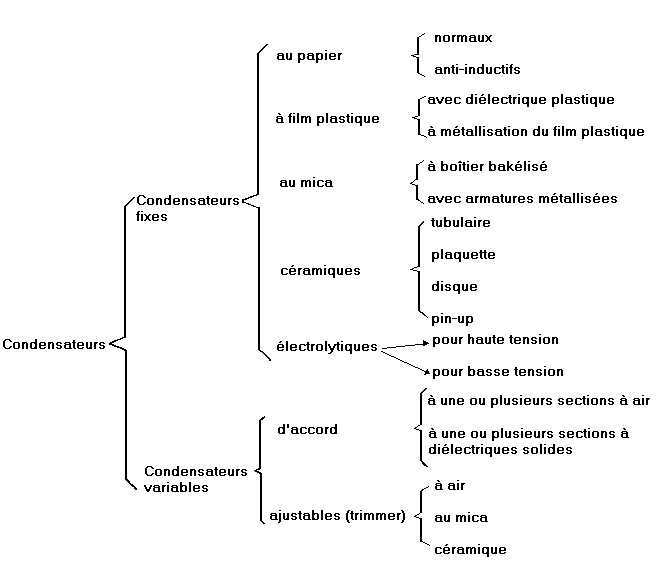
\includegraphics[scale=0.7]{\rootImages/classification.PNG}
    \caption{Classification des différents types de condensateur}
    \label{classification}
\end{figure}

La figure \ref{classification} récapitule tous les types de condensateurs. Ils sont divisés en 2 catégories, les condensateurs à capacité fixes et ceux à capacité variable. Nous allons par la suite nous intéresser majoritairement au condensateur à capacité fixe car ce sont ceux le plus répandus.

\section{Les condensateurs à film}


Ces condensateurs utilisent un film plastique. Il en existe de 2 types, suivant l’utilisation du film plastique.  Ceux de type un utilisent un film plastique comme diélectrique, c’est-à-dire comme moyen de limiter ou empêcher la conduction électrique mais laissant s’exercer les forces électrostatiques. Ceux de type deux utilisent quant à eux un film plastique métallisé. \\


\begin{figure}[!h]
    \centering
    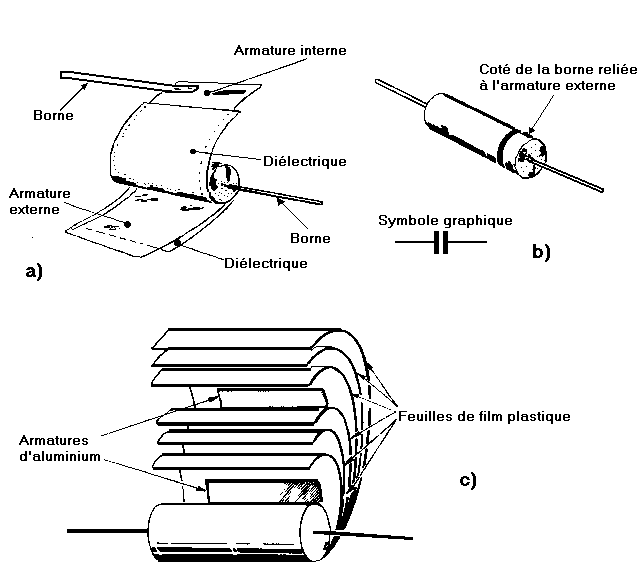
\includegraphics[scale=0.5]{\rootImages/condo_film.png}
    \caption{Schéma interne d'un condensateur à film plastique}
\end{figure}

Ces condensateurs possèdent une faible capacité comprise entre 1nF et 30µF, mais à défaut permettent une très grande précision. Ils possèdent également une durée de vie supérieure à la plupart des autres types de condensateurs et ne sont pas polarisé. De plus, certains de ces condensateurs permettent une régénération après un claquage. Ils sont également conçus pour résister à de hautes tensions (de l’ordre du kilovolt) et permettent de fournir des impulsions de courant de surcharge très élevées.

\newpage
\section{Les condensateurs à céramique}

Ce type de condensateur est celui majoritairement utilisé. Ils sont notamment très utilisés en électronique du fait de leur petite taille. Ils permettent des capacités comprises entre 1nF et 1µF. Ils ne sont pas polarisés comme les condensateurs à film ce qui permet leur utilisation dans des circuits à courant alternatif. Il en existe également 2 types :\\

\begin{itemize}
    \item Ceux de classe 1 sont utilisés lorsque l’on nécessite une grande stabilité et de faible perte. Ils possèdent une valeur de capacité très stable.\\
    \item Ceux de classe 2 possèdent une capacité élevée. Ils perdent cependant en stabilité thermique et les tolérances de capacité sont plus élevée.
\end{itemize}

\begin{figure}[!h]
    \centering
    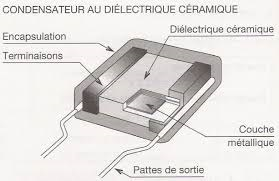
\includegraphics[scale=1]{\rootImages/condo_ceramique.jpg}
    \caption{Schéma interne d'un condensateur à céramique}
\end{figure}


\newpage
\section{Les condensateurs électrolytiques}

Les condensateurs électrolytiques ou encore condensateurs chimiques, utilisent un électrolyte, c’est-à-dire une substance conductrice contenant des ions mobiles. Cela permet à ces condensateurs de pouvoir fournir une plus grande plage de valeur de capacité que les autres types de condensateur. Ils sont dans la très grande majorité polarisé ce qui oblige leur utilisation dans des circuits à courant continu. On en voit très souvent dans des alimentations notamment d'ordinateur etc... Ils permettent une capacité comprise entre 1µF et 47mF avec une tension de fonctionnement pouvant aller à l’ordre de quelques centaines de volts. Ils ne sont cependant pas très précis. En effet il possède une tolérance de 20\%, une grande résistance en série et réagissent très mal aux hautes fréquences (surchauffe). 


\begin{figure}[!h]
    \centering
    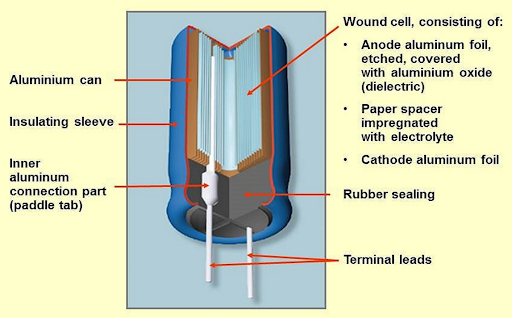
\includegraphics[scale=0.5]{\rootImages/condo_electro.png}
    \caption{Schéma interne d'un condensateur électrolytiques}
\end{figure}


\section{Les condensateurs variables}

Les condensateurs variables sont des condensateurs dont la valeur de la capacité est comme son nom l’indique variable. Ils sont constitués d’un rotor, d’un axe et d’un stator. 

\begin{figure}[!h]
    \centering
    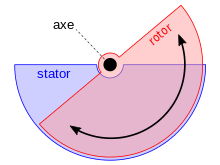
\includegraphics[scale=0.5]{\rootImages/condo_variable.png}
    \caption{Schéma interne d'un condensateur variable}
\end{figure}

Le rotor entraîné par l’axe tourne dans l’armature fixe du stator. La capacité de ces condensateurs varie en continu entre une valeur minimum appelé capacité résiduelle et une valeur maximum appelée capacité nominale. \\

Cette variation suit une fonction appelée loi de variation : 

\begin{align}
    C=f(\theta)
\end{align}

f() dépend de multiples paramètres complexes. Il est donc difficile de pouvoir le définir clairement.\\
$\theta$ quant à lui correspond à l'angle de rotation de l'axe. \\ \\

\begin{figure}[!h]
    \centering
    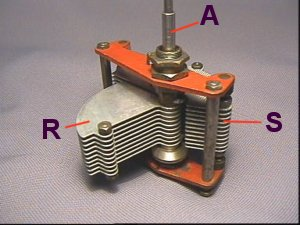
\includegraphics[scale=0.8]{\rootImages/condo_variable.jpg}
    \caption{Condensateur à capacité variable}
\end{figure}


Nous avons pu dans cette partie, nous intéresser à différents types de condensateur. Il en existe encore plein d'autres comme les condensateurs au mica, au papier... Mais nous avons vu ici, ceux les plus couramment utilisés.
\chapter{Domaines d'application}


Nous allons présenter trois domaines d'application des condensateurs. Cette liste n'est pas exhaustive. Les condensateurs permettent également de redresser le cosinus $\Phi$ ou bien de filtrer des signaux audio.

\section{Les condensateurs de filtrage}

\subsubsection{Présentation}

Les condensateurs permettent de lisser une tension afin de stabiliser cette dernière.

\subsubsection{Objectif}

On souhaite amortir les oscillations de tension en sortie d'un pont de Graëtz (14 V DC).\n
On souhaite donc passer d'une tension alternative à une tension pseudo-continue.

\img{\rootImages/graetz}{Le pont de Graetz}{0.5}

\img{\rootImages/graetz_input}{La tension en sortie du pont}{0.5}



\subsubsection{Mise en oeuvre}

Afin de lisser la tension, il convient de mettre un condensateur en sortie du pont de Graëtz, avec une borne sur INPUT et une autre à la masse. \n 
Une résistance de 50 $\Omega$ a été rajoutée pour simuler la présence d'une charge.

\img{\rootImages/out_filtre.png}{Le circuit de filtrage }{0.5}

Observons le résultat.

\img{\rootImages/graetz_out}{La tension aux bornes du condensateur }{0.7}

\subsubsection{Principe}

Le condensateur joue le rôle d'accumulateur. Pendant les phases ou la tension est croissante, ce dernier se charge. \n 
Lors des phases ou la tension décroît, le condensateur restitue une partie de son énergie, ce qui a pour effet de réduire l'amplitude de variation de tension.\n 

On retrouve notamment ces condensateurs dans les alimentations linéaires. \n 
Dans ce cas, la capacité du condensateur nécessaire croit avec le courant demandé par la charge. \n 

Il est fréquent de voire des condensateurs chimiques de quelques mF dans ces alimentations. Une valeur inférieure risque de rendre instable l'alimentation.







\section{Les condensateurs de découplage}

\subsubsection{Présentation}


Certains circuits nécessitent une alimentation très stable (aucune fluctuation de la tension d'entrée). Cependant, lors de l'utilisation du circuit, des courants importants peuvent être demandés par le circuit. \n
Nous allons montrer un cas en exemple où, pour améliorer les performances du circuit, il conviendra de mettre de fameux condensateur de découplage.

\subsubsection{Objectif}

Nous souhaitons cascader deux portes logiques CMOS\footnote{Complementary MOS : MOS complémentaires, mise en cascade d'un MOS canal P et d'un MOS canal N} de type inverseur, comme le montre la figure suivante.

\img{\rootImages/cmos_purpose.png}{Schéma d'exploitation}{0.3}

A première vue, ce modèle peut sembler satisfaisant. Cependant, nous souhaitons faire fonctionner ce circuit dans des fréquences assez élevée \footnote{Toutefois inférieures à la fréquence maximale du circuit}.

En prenant un modèle réel, on peut déjà prendre en compte les capacités parasites des transistors MOSFETs. Ces derniers possèdent une capacité entre la broche de commande (Gate) et la masse. \n

Le modèle réel des entrées de chaque porte logique est le suivant.

\img{\rootImages/real_input_cmos.png}{Modèle équivalent des entrées CMOS}{0.3}


\subsubsection{En régime transitoire}
Intéressons nous au régime transitoire. \n
On constate que dans notre cas d'exemple, les grilles des  MOSFETS consomment du courant pendant les phases de commutation, du fait qu'il faut charger ou décharger les condensateurs.
Cet appel de courant peut faire réduire la tension d'alimentation si cette dernière n'est pas très puissante.


\subsubsection{En régime stationnaire}

Lorsque la tension d'entrée (INPUT) est constante et que le condensateur est chargé (ou déchargé), les grilles des MOSFETs ne sont parcourus par aucun courant \n

\subsubsection{Le modèle réel}

L'alimentation étant rarement en liaison directe avec le circuit logique (piste de circuit imprimé, fils d'alimentation), on constate l'apparition d'une inductance parasite entre la borne d'alimentation du circuit et l'alimentation en elle-même.
Le modèle équivalent final du circuit peut être modélisé par la figure suivante.

\img{\rootImages/noise.png}{Modèle équivalent du circuit}{0.3}

L'inductance parasite s'oppose aux variations de tensions. \n Ainsi, lors des phases de commutation (régime transitoire), une partie de la tension d'alimentation va au bornes des inductances parasites.
De ce fait, le circuit est de moins en moins efficace à mesure que l'on augmente la fréquence du signal d'entrée.
Pour pallier à ce problème, nous allons ajouter un condensateur de découplage.
\subsubsection{Mise en oeuvre du condensateur de découplage}


Le condensateur de découplage doit être placé au plus près du circuit à alimenter. Une de ses bornes est reliée à la broche d'alimentation du circuit et la seconde à la masse. \n

\img{\rootImages/capa_decouplage.png}{Le placement du condensateur de découplage}{0.5}

Lorsque le circuit en aval va demander du courant lors des commutations, le condensateur, qui va se charger pendant le régime permanent du circuit, va pouvoir fournir un apport de courant qui évitera à la tension d'alimentation de s'écrouler. Le circuit sera plus efficace et les temps de communication seront plus faibles. \n


D'un point de vue des filtres, ces condensateurs peuvent être considérés comme des filtres passe-bas. En effet, la tension d'alimentation qui varie est vue comme un signal haute fréquence. Il faut donc éviter l'oscillation haute fréquence.

\section{Les condensateurs de liaison}

\subsubsection{Présentation}

Une des propriétés des condensateurs est de bloquer les composantes continues.
Nous allons aborder un exemple ou le condensateur va permettre de se passer d'une alimentation symétrique. 

\subsubsection{Objectif}

On souhaite amplifier la composante alternative d'un signal d'amplitude 1V, de tension moyenne 0.5V et de fréquence 1kHz avec un AOP alimenté en 0-12V (Alimentation asymétrique).

\img{\rootImages/sinus.png}{Le signal à amplifier}{0.6}

\subsubsection{Mise en oeuvre}

Tout d'abord, on va chercher à recentrer le signal pour avoir une composante alternative toujours positive.
Pour cela, on utilise le circuit suivant.

\img{\rootImages/bridge.png}{Montage pour recentrer la tension}{0.4}

La fréquence de coupure valant $\frac{1}{2\pi RC}$ avec $ R < 10 k\Omega$, il faudra prendre un condensateur tel que la fréquence de coupure soit inférieure à la fréquence du signal d'entrée. \n
Un condensateur de 1 mF conviendra donc pour cette application.\n

En utilisant le théorème de superposition au point OUTPUT, on en déduit que une résistance de $10 k\Omega$ et une résistance de $ 900 \Omega$, on obtient la tension OUTPUT suivante.

\img{\rootImages/bridge_level.png}{Tension positive}{0.5}

Il nous reste à amplifier la tension OUTPUT (ici par 2). Nous obtenons donc une tension sinusoïdale d'amplitude 2V. \n

\img{\rootImages/bridge_output.png}{Schéma avec les deux condensateurs de liaison}{0.7}

Pour extraire la composante alternative, il suffit de mettre en sortie un condensateur qui va recentrer le signal en 0V.
Le condensateur sera de 1mF (même fréquence). \n
Nous obtenons finalement un signal de sortie avec un gain de 2 de la composante alternative d'entrée.\n

\img{\rootImages/vs_liaison.png}{La tension de sortie}{0.6}
Au final, les deux condensateurs permettent à des portions de circuits de communiquer entre elles avec des niveaux de tension différents. Ces condensateurs sont appelés \textbf{condensateurs de liaison ou de couplage}\chapter{Avenir du condensateur}

Nous avons donc vu dans les parties précédentes que le condensateur est un élément essentielles à tout circuits électronique. Nous nous sommes donc posé la question suivante : Le condensateur sera-t-il amené à disparaître dans le futur pour être remplacé par un autre composant ?
Il est évident que l'importance du condensateur est telle qu'il parait irremplaçable. En effet, on ne peut se passer d'un telle composant dans un circuit électronique. Cependant, depuis quelques années un composant est utilisé de plus en plus : le super-condensateur. 

\section{Les supercondensateurs}

Les supercondensateurs sont une sous-catégorie des condensateurs électrolytiques. Ils permettent de stocker une très grande quantité d’énergie grâce à une combinaison de 2 technologies de capacité. La capacité double couche que l’on retrouve dans les condensateurs électrolytiques et la pseudo-capacité. L’une est électrostatique et l’autre électrochimique.

\img{\rootImages/supercondensateurs-lithium-ion-avenir-stockage-Les-Smart-Grids-2}{La description de l'image}{0.5}
Cela leur permet de combiner les caractéristiques des condensateurs ordinaires et celles des batteries. En effet grâce à ces technologies ils peuvent atteindre des capacités allant jusqu’à 12 000F, tout en ayant des temps de charge et décharge très rapide comparable aux condensateurs ordinaires. Toutes ces caractéristiques en feraient de bons candidats pour remplacer nos batteries au lithium. Mais c’était sans compter leurs défauts. Ils sont en effet très chers à produire, possèdent une faible énergie spécifique (Rapport en Wh/kg entre l’énergie électrique fournie par unité de temps et la masse du convertisseur) et une tension de décharge linéaire. Cela entraînerait de grandes chutes de tension d’alimentation très rapidement.
Le supercondensateur sera probablement l'avenir pour le stockage d'électricités, qui a terme remplacera sûrement les batteries des véhicules électriques. Cependant, il est trop puissant pour le mettre dans la majorité des circuits électroniques. La science progresse énormément dans ce domaine.

\chapter{Introduction}

\addQuote{En dépit des perfectionnements électroniques, il advient parfois que la bonne vieille feuille imprimée soit le moyen d’information le plus pratique.}{Arthur Charles Clarke}


Pour certains projets plus évolués, on souhaite utiliser des composants tels que des moteurs ou des résistances (chauffage, ventilation).
Or, on constate rapidement que le branchement direct de ces éléments sur une carte Arduino va se révéler impossible. \\

En effet, la carte Arduino est prévu pour délivrer de \bold{faibles courants} et \bold{faibles tensions}.

Nous allons donc créer un circuit où la puissance et la commande sont dissociés.

\chapter{Les transistors bipolaires}

\section{Présentation}

Une des moyens pour créer notre circuit de puissance est le transistor bipolaire.
Ce composant possède trois broches : 

\begin{itemize}

  \item Le collecteur (C)
  \item la base (B)
  \item l'émetteur (E)

\end{itemize}

\img{\rootImages/bjt}{La représentation du transistor bipolaire}{0.2}

\section{Conventions}

Afin de simplifier les calculs par la suite, posons les normes suivantes : 

\begin{itemize}

  \item Le courant entrant dans le Collecteur est appelé $I_{C}$
  \item Le courant entrant dans la Base est appelé $I_{B}$
  \item Le courant sortant de l'émetteur est appelé $I_{E}$

  \item La tension entre la Base et l'Emetteur est appelée $V_{be}$
  \item La tension entre le Collecteur et l'Emetteur est appelée $V_{ce}$
\end{itemize}

\img{\rootImages/courants}{Conventions du transistor bipolaire}{0.15}


Les flèches au sein du transistor indiquent le sens de déplacement du courant sur les broches.

\subsection{Les familles de transistors bipolaires}

Les transistors bipolaires sont classés en deux catégories : 

\begin{itemize}

  \item Les transistors NPN\footnote{Le nom de ces familles provient du type de jonction utilisé en interne. Pour plus de rensiegnement, consulter les diodes et semi-conducteurs}
  \item Les transitors PNP

\end{itemize}

Le principe de fonctionnement est similaire entre ces deux familles, seul le branchement et le niveau de commande diffère.\\
Dans ce document, nous utiliserons essentiellement des transistors NPN car ces derniers utilisent des grandeurs positives.

\img{\rootImages/pnppnp}{Transistors NPN et PNP}{0.6}


\section{Les paramètres de sélection du transistor}

Notre transistor doit dans un premier temps répondre à deux contraintes : 

\begin{itemize}

  \item La tension admissible sur $V_{ce}$\footnote{Cette tension est indiquée ddans les documentations techniques} doit être supérieur à la tension d'alimentation de notre circuit.
  Concrètement, si notre circuit est alimenté en 48V mais que le transistor ne supporte pas plus de 30V, il va être détruit.
  \item Le transistor doit supporter un courant plus élevé que le courant maximal transitant dans notre circuit.
  Pour contrôler un moteur consommant 1 Ampère, je dois donc choisir un transistor pouvant contrôler au moins 1 Ampère.
\end{itemize}

Pour la suite de la présentation, on supposera que notre transistor a été dimensionné pour répondre à ces deux contraintes.


\section{Le principe}

Ce type de transistor fonctionne comme une vanne pour une canalisation. Il est possible de réguler le débit de la canalisation avec la vanne. \\

Le transistor bipolaire permet de contrôler un courant important avec un faible courant.\\

\img{\rootImages/barrage.png}{Le rôle du transistor}{0.3}.

Ici, notre transistor joue le rôle de la vanne et permet de bloquer le courant (électrons) ou bien de les laisser passer. \\


Le courant de l'élément à contrôler (moteur, résistance de puissance....) transite entre le collecteur et l'émetteur et le courant de commande passe par la base, comme l'illustre la figure suivante.\\

\img{\rootImages/courant_main.png}{Courant de commande et de puissance}{0.6}

La relation fondamentale reliant le courant de puissance et de commande est la suivante : 

$$ \boxed{ I_{C} = \beta \cdot I_{B} }$$

Le paramètre $\beta$, appelé \bold{gain du transistor}\footnote{le gain est sans dimension (unité) et est appelé \italic{$h_{fe}$} dans les documentations} est une caractéristique interne de notre transistor, c'est à dire qu'il dépend du type de transistor que nous choisissons.\\
Les courants $I_{C}, I_{B},I_{E}$ sont exprimés dans la même unité (Ampère, milliampères..) pour une formule homogène.\\

Les transistors de puissance possède des gains de l'ordre de la dizaine alors que les transistors de signal (faibles courants) ont un gain pouvant facilement atteindre 200 ou 300.

\messageBox{Remarque}{cyan}{white}{Plus notre $\beta$ est faible, plus il va falloir injecter un courant important dans notre base}{black}

\begin{question}
  Et que devient notre broche "\bold{Émetteur}" ?
\end{question} 

\begin{reponse}
  
  Notre émetteur est relié à la masse du circuit et permet de le fermer pour que les électrons puissent circuler.\\

  Le courant circulant dans l'émetteur est simplement la somme des courants entrant dans le transistor. \\
  d'où : $$ \boxed{ I_{E} = I_{B} + I_{C} }$$

  \end{reponse}



\section{Exemple}

On souhaite commander l'arrêt et la marche d'un moteur consommant au maximum 0.5A et alimenté avec une tension de 9V. \\
Nous choisissons un transistor permettant de commuter 1A (sécurité) avec $\beta=30$ \\

\begin{question}
Quel doit-être le courant injecté dans la base ?
\end{question}

\begin{reponse}
  On applique la formule précédent et on obtient : 

  $$  I_{B} = \frac{I_{C}}{\beta} = \frac{0.5}{30} = 16 mA $$

  \end{reponse}

 

    \section{Mise en pratique}

    \subsection{Branchements}

    Maintenant que nous connaissons les tensions et courants nécessaires à notre transistor et à notre moteur, nous allons le commander avec une carte Arduino. \\

    Tout d'abord, il convient de placer le moteur entre notre alimentation et le collecteur.\\
    

     \messageBox{Remarque}{cyan}{white}{{\color{red}Toutes les charges à contrôler avec ce type de transistor se placent entre l'alimentation et le collecteur.}}{black}

    Enfin, il ne nous reste plus qu'à relier une sortie numérique de l'Arduino vers notre base par l'intermédiaire d'une résistance.

    \bold{La résistance va servir à imposer le courant dans la base de notre transistor}.

    Nous obtenons donc le schéma suivant.

    \img{\rootImages/schema_pnp.png}{Branchement du transistor bipolaire}{0.4}

    \subsection{Dimensionnement de la résistance}

    On souhaite obtenir un courant de $16 mA$ dans notre base et on sait que l'Arduino délivre du $5V$ en sortie.\\

    Nous somme donc tentés de dire que $R_b = \frac{U_{arduino}}{ I_{B}} = \frac{5}{0.016} = 312 \Omega$ \footnote{On part de la loi d'Ohm qui dit que $U=R.I$}\\


    Hélas, il y a peu de chance que votre moteur tourne dans les conditions optimales.\\
    Il convient d'avoir à l'esprit que notre $\beta$ trouvé dans la documentation n'est que théorique et qu'il peut être en réalité inférieur.

    \messageBox{Remarque}{cyan}{white}{Une des conventions non officielles admet que pour de la commutation en \bold{Tout ou Rien}\footnote{Le transistor laisse passer tout le courant nécessaire ou rien du tout}, on divise la valeur théorique de notre $\beta$ par 2. \\Nous allons donc prendre donc un $\beta$ valant 15.}{black}
    
    On refait donc les calculs.

    $$  I_{B} = \frac{I_{C}}{\beta} = \frac{0.5}{15} = 32 mA $$

    Une dernière chose : les transistors bipolaires entraînent une chute de tension entre la base et l'émetteur ($V_{be}$).\\
    Cette chute de tension dépend de la technologie des transistors bipolaires : 

    \begin{itemize}

      \item $0.7V$ pour les transistors au silicium
      \item $0.3V$ pour les transistors au germanium
    \end{itemize}
    Dans l'extrême majorité des cas, on utilisera des transistors au silicium.

    La tension disponible aux bornes de la résistance est donc de $4.3V$ ($5-0.7$)

    D'où : 

    $$ \boxed{ R_{b} = \frac{U_{arduino}-V_{be}}{I_b} = \frac{4.3}{0.032} = 134 \Omega} $$

    \subsection{Exemple de programme Arduino}

    Voici un code permettant de faire tourner le moteur périodiquement pendant 5 secondes puis de l'arrêter pendant 5 secondes.

\begin{Cpp}{Code Arduino avec transistors NPN}
#define D8 8     //Broche 8 de l'Arduino

void setup() {

  pinMode(D8, OUTPUT); //Mise en sortie de la broche

}//End setup

void loop() {

  digitalWrite(D8, HIGH);     //Déclencher la rotation du moteur
  delay(5000);                //Délai de 5s
  digitalWrite(D8, LOW);      //Fin de la rotation du moteur
  delay(5000);                //Délai de 5s

}//End loop

\end{Cpp}

     \chapter{Les transistors MOSFET}

     \section{Présentation}

     Nous avons vu l'utilisation des transistors bipolaires. \\
     Ces derniers sont assez contraignants à mettre en oeuvre car ils sont commandés en courant.

     Nous allons utiliser cette fois-ci la technologie des MOSFET \footnote{MOSFET : Metal Oxide Semiconductor Field Effect Transistor = Transistor à effet de champ à structure métal-oxyde-semiconducteur} car ces derniers ont l'avantage d'être contrôlés en \bold{tension}.

     Ce composant possède trois broches : 
     
     \begin{itemize}
     
       \item Le drain (D)
       \item la porte (G)\footnote{'G' pour Gate}
       \item la source (S)
     
     \end{itemize}
     
     \img{\rootImages/mosfet.png}{La représentation du transistor MOSFET}{0.1}
     
     \section{Conventions}
     
     Afin de simplifier les calculs par la suite, posons également les normes suivantes : 
     
     \begin{itemize}
     
       \item Le courant entrant dans le Drain est appelé $I_{D}$
       \item Le courant entrant dans la Porte est appelé $I_{G}$
       \item Le courant sortant de la Source est appelé $I_{S}$

       \item La tension entre la Porte et la Source est appelée $V_{GS}$
       \item La tension entre le Drain et la Source est appelée $V_{DS}$
     \end{itemize}
     
     \subsection{Les familles de transistors MOSFET}

     Les transistors MOSFET sont classés en deux catégories : 
     
     \begin{itemize}
     
       \item Les transistors MOSFET à canal N\footnote{Le nom de ces familles provient du type de jonction utilisé en interne. Pour plus de rensiegnement, consulter les diodes et semi-conducteurs}
       \item Les transitors MOSFET à canal P
     
     \end{itemize}
     
     Le principe de fonctionnement est similaire entre ces deux familles, seul le branchement et le niveau de commande diffère.\\
     Dans ce document, nous utiliserons essentiellement des transistors MOSFET à canal N car ces derniers utilisent des grandeurs positives.
     
     \img{\rootImages/mos.png}{Transistors à canal N et P}{0.6}

     \section{Les paramètres de sélection du transistor}
     
     Les paramètres de sélection de nos transistors MOSFET sont identiques aux transistors bipolaires, c'est à dire :
     
     \begin{itemize}
     
       \item La tension admissible sur $V_{DS}$ du transistor
       \item Le courant admissible entre le Drain et la Source.
     \end{itemize}
     
     Pour la suite de la présentation, on supposera que notre transistor a été dimensionné pour répondre à ces deux contraintes.


     \section{Le principe}

     Ce type de transistor fonctionne comme les transistors bipolaires mais est commandé en tension et non en courant.

     Par analogie, le drain joue le rôle du collecteur, la source celui de l'émetteur et la porte celui de la base.
     Le courant de l'élément à contrôler (moteur, résistance de puissance....) transite entre le drain et la source et la tension de commande est aux bornes de la porte.\\
     
     Les transistors MOSFET deviennent passant\footnote{Le transistor laisse passer tout le courant autorisé.} lorsque la tension sur la porte dépasse une tension de déclenchement appelée $V_{GS_{th}}$.
     Cette valeur est généralement comprise entre $2$ et $4$ Volts.\footnote{Lorsque la tension $V_{GS}$ est inférieure à $V_{GS_{th}}$, $I_D$ vaut $K \cdot ( (V_{GS}-V_{th})\cdot V_{DS}-\frac{1}{2}V_{DS}^2)$ \\Cette relation montre que l'étude en amplification est plus complexe car non linéaire.}\\

     \bold{Lorsque cette tension $V_{GS_{th}}$ est atteinte, notre transistor peut être remplacé d'un point de vue électrique entre le drain et la source par une résistance de très faible valeur, appelée $R_{DS_{on}}$}

    \section{Comparaison avec les transistors bipolaires}

    Par nature, la porte du MOSFET est vue comme un condensateur. Le transistor ne consomme pas de courant, excepté pendant les commutations.\\
    Ainsi, le courant est nul dans la porte pour maintenir le moteur en marche alors que pour un bipolaire, il faut maintenir un courant dans la base.\\

    Les MOSFET sont donc plus économes en énergie que les bipolaires.\\
    De plus, ils peuvent généralement supporter des courants plus importants que les bipolaires.\\

    En revanche, en hautes fréquences, les MOSFET sont moins réactifs du fait de leur capacité en entrée.
     \section{Mise en pratique}

     Nous souhaitons faire tourner le même moteur que celui utilisé avec notre transistor bipolaire.\\
     Nous allons le commander avec une carte Arduino.

     \subsection{Branchements}

     Tout d'abord, il convient de placer le moteur entre notre alimentation et le drain.\\
     
 
    \messageBox{Remarque}{cyan}{white}{{\color{black}Toutes les charges à contrôler avec ce type de transistor se placent entre l'alimentation et le drain.}}{black}
 
     Enfin, il ne nous reste plus qu'à relier une sortie numérique de l'Arduino vers notre porte \bold{sans} résistance.
 
     Nous obtenons donc le schéma suivant.
 
     \img{\rootImages/schema_mosfet.png}{Branchement du transistor MOSFET}{0.45}
  
     \subsection{Exemple de programme Arduino}
 
     Voici un code permettant de faire tourner le moteur périodiquement pendant 5 secondes puis de l'arrêter pendant 5 secondes. Il s'agit du même code que pour le transistor bipolaire.
 
 \begin{Cpp}{Code Arduino avec MOSFET}
 #define D8 8     //GATE du transistor
 
 void setup() {
 
   pinMode(D8, OUTPUT); //Mise en sortie de la broche
 
 }//End setup
 
 void loop() {
 
   digitalWrite(D8, HIGH);    //déclenchement du moteur
   delay(5000);               //Délai de 5s
   digitalWrite(D8, LOW);     //arrêt du moteur
   delay(5000);               //Délai de 5s
 
 }//End loop
 
 \end{Cpp}

 \chapter{Conclusion}

 \section{Ce qu'il faut retenir}

 
 Nous avons à notre disposition tout un ensemble de technologies pour contrôler la partie puissance.

 Les transistors ne sont pas adaptés pour commuter une charge sur secteur (230V), cette partie sera donc réservée aux relais.\\
 En revanche, pour toutes les tensions continues, les transitors sont adaptés et prennent moins de place en encombrement.\\

 \section{Les fiches techniques}

 L'intégralité des informations disponibles pour un transistor sont disponibles dans un document complet appelé \bold{Datasheet}.

 Ce document détaille les broches, les caractéristiques électriques, propose des schémas d'exemples....\\

 Par exemple, voici quelques extraits de la documentation du transistors IRF520\footnote{Transitor de puissance} :

 \img{\rootImages/irf520.png}{Extrait n°1 du IRF520}{0.4}

 \img{\rootImages/rdson.png}{Extrait n°2 du IRF520}{0.5}

 On retrouve sur cette figure la valeur de $R_{DS_{on}}$ et de $V_{GS_{th}}$

\chapter{Les familles des circuits logiques}

\section{Présentation}

Les circuits logiques sont des éléments permettant de réaliser des opérations avec l'algèbre de Boole (uniquement des '0' et des '1').
Pour réaliser ces opérations (ET, NON, OU, NON-OU, NON-ET...), des circuits ont vu le jours dans les années 60 avec deux grandes familles de circuits : \\
\begin{itemize}
    \item La famille TTL
    \item La famille CMOS
\end{itemize} 


De nouvelles technologies arrivent à maturité mais nous ne les évoquerons pas ici.

\subsection{Principe TTL}

Les circuits TTL sont composées de transistors bipolaires NPN ou PNP. \\
Les transistors bipolaires sont commandés en courant.


\subsection{Principe CMOS}

La famille CMOS, quant à elle, repose sur l'utilisation en interne de transistors MOS complémentaires (C). \\
Les transistors MOS, du fait de leur structure, sont commandés en tension.


\section{Comment les distinguer ?}

La famille des CMOS est rapidement identifiable car le nom du composant contient un numéro commençant par 40 et se termine avec un nombre à 2 ou 3 chiffres (40XX ou 40XXX). \\

Par exemple, CD4001, CD4017 sont des composants CMOS. \\



La famille des TTL contient en général le chiffre 74\footnote{La série militaire des TTL possède le numéro 54 et possède de meilleurs caractéristiques : plage de température de fonctionnement plus élevée, fréquence plus élevée...} encadré par des lettres et des chiffres. \\





\section{Avantages et inconvénients}

\begin{itemize}
    \item Les TTL consomment plus de courant que les CMOS \footnote{Ces derniers consomment uniquement lors des phases de commutation}
    \item Les CMOS ont des fréquences de fonctionnement plus faibles que les TTL.
\end{itemize}

\chapter{Les signaux}

\section{Introduction}

Un signal est une évolution d'une grandeur physique.\\
Il permet donc de caractériser cette grandeur qui peut ensuite être traitée par un circuit adapté.


\begin{itemize}
    \item Les signaux numériques
    \item Les signaux analogiques
\end{itemize} 

\subsection{Les grandeurs physiques}

Afin de mieux comprendre comment un signal peut se former, nous allons étudier les notions de tensions, de courant et de résistances électriques.
Pour cela, plongeons nous dans la matière, au niveau des électrons

\subsection{Les atomes}

\subsection{La charge électrique}

%\box{La charge est exprimée en Coulomb}

\subsection{Les électrons}

Les électrons forment la couche extérieure de l'atome, élement insécable de notre univers.

%image atome.

Lorsqu'un électron se déplace dans l'espace, ce dernier engendre un courant.

%\box{Le courant électrique est le nombre d'éléctrons par unité de temps}
\boxed{Le~courant~électrique~est~le~nombre~d'éléctrons~par~unité~de~temps}


La charge électrique représente quant à elle le nombre d'électron à un endroit donné et à un temps précis.

\section{La tension électrique}

Nous avons vu que le courant est une nombre de charges par unité de temps. \\
Comment pouvons nous engendrer ce courant ? Tout simplement en soumettant une différence de potentiel, autremeent dit une \bold{tension}

\section{Analogie}
\newcommand{\A}{$A~$}
\newcommand{\B}{$B~$}

Afin de mieux comprendre ce principe, faisont une analogie.

Prenons un rivière, un barrage et une montagne.

Soit deux points sur une route dont nous pouvons régler la hauteur en chaque point. On considère une goutte d'eau entre ces points. \\
Notre objectif est de déplacer notre goutte d'un point à l'autre.

>> Comment faire ?

En surelemavtn le point \A et en abaisant notr point \B, notre goutte va descendre du point le plus élevé au plus bas.

Le courant fonctionne de la même manière : 

\bold{Il ira toujours du potentiel le plus haut au plus faible.}

Pour la petite histoire, historiquement, le sens du courant étaient du potentiel le plus elevé au plus faible.
Bien des années plus tard, les scientifiques se sont rendu compte que le courant allait en réalité du
potentiel le plus faible au plus elevé. Néanmoins, la convention a été gardée...


\subsection{Exemples}
\begin{question}
Soient \A et \B nos deux points du circuits. Ces deux points sont soumis à une tension $U_A$ et $U_B$\\
Quel est le sens de parcours du courant (de \A vers \B, de \B vers \A ou bien autre chose) ?

\begin{figure}[!h]
    \centering
\begin{tabular}{|c|c|c|}
    \hline
    $U_A$ (V) & $U_B$ (V) & Sens du courant ?\\
    \hline
    10 & 5 & \\
    \hline
    5 & 10 & \\
    \hline
    5 & 5 &\\
    \hline
\end{tabular}
\caption{Question sur le sens du courant en fonction des tensions $U_A$ et $U_B$}
\end{figure}
\end{question}
 

\section{Introduction}


Il existe deux grandes familles d'alimentations : 

\begin{items}{orange}{\Triangle}
    \item Les alimentations linéaires
    \item Les alimentations à découpages
\end{items}

Les alimentations linaires sont réputées pour avoir une tension stable et propre (tension continue).\\
Regardons de plus près le principe de ces alimentations.

\section{L'objectif}

On souhaite transformer une tension sinusoïdale\footnote{De valeur efficace 230V et de fréquence 50 Hz} en une tension continue, stable et régulée.

\vfill
\begin{graphicFigure}{0.8}{1}{0}{0.08}{-230}{230}{t(s)}{Tension (V)}{Les tensions d'entrée et de sortie de notre alimentation}
  \addTrace{blue}{0}{0.08}{230*sin(50*360*\x)}
  \addTrace{orange}{0}{0.08}{12}
  \addTrace{black}{0}{0.08}{0}
  \addLegend{Entrée, Sortie, 0V}
  \end{graphicFigure}

  \newpage
  \section{Le choix du transformateur}

  Pour notre circuit, nous devons connaître la tension finale en sortie de notre alimentation.\\
  Au vue des composants demandés (régulateurs, pont de diode), il faudra une tension efficace de $12V$\footnote{Nous verrons la justification de cette valeur par la suite.}
  Le rapport des bobines de notre transformateur sera donc au minimum de \bold{19}. \\Cela veut dire que pour 19 enroulements dans la bobine primaire, il en faudra une seule dans la bobine secondaire.

  La puissance demandée pour le transformateur n'est pas critique, la puissance absorbée par le circuit en aval est négligeable.

  Notre transformateur va donc abaisser la tension du secteur en une tension plus faible.

  \begin{graphicFigure}{0.6}{0.6}{0}{0.08}{-230}{230}{t(s)}{Tension (V)}{Les tensions d'entrée et de sortie du transformateur}
    \addTrace{blue}{0}{0.08}{230*sin(50*360*\x)}
    \addTrace{red}{0}{0.08}{14*sin(50*360*\x)}
    \addTrace{black}{0}{0.08}{0}
    \addLegend{Entrée, Sortie, 0V}
    \end{graphicFigure}

    \newpage 
  \section{Le pont redresseur de tension}

  \subsection{Principe}
  Notre objectif est maintenant de supprimer la composante négative de notre signal. Pour cela, on va utiliser la propriété des diodes qui ont la faculté de laisser passer le courant dans un seul sens.\\
  Un montage existant est le Pont de Graetz.

  \img{\rootImages/diode.png}{Le pont de diode}{0.5}

  Observons le résultat lorsque nous mettons notre tension de sortie du transformateur sur notre entrée de pont.

  \begin{graphicFigure}{0.6}{0.6}{0}{0.08}{-20}{20}{t(s)}{Tension (V)}{Les tensions d'entrée et de sortie du pont de diode}
    \addTrace{blue}{0}{0.08}{12*sin(50*360*\x)}
    \addTrace{red}{0}{0.08}{abs(15.64*sin(50*360*\x))}
    \addTrace{black}{0}{0.08}{0}
    \addLegend{Entrée, Sortie, 0V}
    \end{graphicFigure}

  On constate que la tension de sortie est plus élevée que notre tension d'entrée.\\
  Cette valeur s'explique par les diodes. 
  
  En sortie, nous voulons une tension de $15V$. Or, les $12V$ en entrée de notre pont sont une valeur efficace, ce qui veut dire que la valeur réelle vaut $17.04V$
    En effet : 
  $$V_{réelle} = V_{efficace}\cdot \sqrt{2} = 12\cdot 1.41 = 17.04 V$$

  Or, à chaque changement de polarité dans notre pont (signal alternatif [positif et négatif]), le courant passe à travers deux diodes.\\

  Chaque diode engendre une chute de tension de $0.7V$, d'où une perte de $1.4V$ en sortie.

  Nous avons comme tension finale en sortie de pont: 

  $$V_{s} = V_{efficace}\cdot \sqrt{2} - 0.7\cdot 2 = 12\cdot 1.41 -1.4 = 15.64 V$$


  \subsection{Un exemple de boîtier}

    La plupart des boîtiers possèdent 4 broches

    \begin{items}{blue}{\Triangle}
      \item deux broches $V_{~}$ pour la tension alternative
      \item Une broche $V_-$ pour la masse du circuit en aval
      \item Une broche $V_+$ pour la tension positive du circuit en aval
   \end{items}

  \img{\rootImages/case.png}{Un exemple de boîtier}{0.2}


  \section{Les condensateurs}

  \subsection{Principe}
  Comme vu à la section précédente, notre signal n'est pas continu et possède des oscillations élevées.
  Nous cherchons à produire une tension continue.\\

  Pour cela, nous allons utiliser des condensateurs.\\

  Leur rôle sera d'accumuler de l'énergie lorsque le signal monte en amplitude et de restituer cette énergie lorsque le signal sera sur sa phase descendante.

  \img{\rootImages/signal.png}{Le rôle du condensateur}{0.6}

  \subsection{Choix de la valeur}
  Plus la valeur du condensateur est élevée, plus notre signal sera lisse en sortie, ce qui est l'effet recherché.\\
  En effet, la capacité du condensateur exprime la quantité d'énergie emmagasinée dans le condensateur.\\

  Un condensateur de $1mF$ et plus est une valeur normale.\\
   Une fois notre tension assez propre (même si elle présente des oscillations), nous allons utiliser les régulateurs de tensions.

  \section{Les Régulateurs de tension}

  \subsection{Principe et branchements}
  Ces composants à trois broches servent à stabiliser une tension pseudo-continue en une tension continue et stable, c'est à dire ne présentant pas d'oscillations.\\


  Le branchement est le suivant : \\

  \img{\rootImages/lm.png}{Un régulateur de tension}{0.8}

  \begin{items}{blue}{\Triangle}
    \item L'entrée INPUT est la tension à réguler
    \item La broche GROUND est la masse du circuit
    \item la sortie OUTPUT est la tension regulée (stable)
\end{items}

\subsection{Les familles des régulateurs}

  Il existe différentes familles de régulateurs linaires, les plus connus étant les LM78XX\footnote{XX prend la tension régulée de sortie (5,9,12,15,18V...)} ou les LM317 qui sont des régulateurs de tension réglables.\\
  Pour des tensions négatives, se référer à la famille des LM79XX.\\

  Pour que ces composants fonctionnent correctement, il convient de leur mettre en entrée une tension supérieure à leur tension de régulation.\\

  Concrètement, si on utilise un LM7812 (régulateur 12 V), il faudra mettre en entrée au moins 15 V pour que le composant fonctionne dans la plage idéale.\\

  \bold{Cette tension de $15V$ justifie la valeur de tension du transformateur.}

  Ces composants sont linéaires, c'est à dire que la différence de tension entre l'entrée et la sortie ($V_{e}-V_s$) engendre une perte de puissance dans le système.\\
  Cette perte dépend directement du courant absorbé par le circuit en aval mais également de la différence de tension $(V_e-V_s)$.\\
  Cette puissance vaut : $$ P_{perdue} =(V_e-V_s)\cdot I_{charge} ~~~~(W)$$

  \subsection{Un exemple}

  On souhaite réguler un circuit en 12V, ce dernier consommant 150 mA ($I_{charge}$).

  La perte d'énergie vaut $$ P_{perdue} =(V_e-V_s)\cdot I_{charge} =(15-12)\cdot 0.150 = 0.45 W$$

  % \subsection{la résistance thermique des régulateurs}

  % En fontion de cette puissance perdue, il est possible de calculer l'élevation de la température du régulateur de tension.

  % La documentation technique des régulateurs de tension précise la valeur de la résistance thermique, c'est à dire de l'élévation de température lorsque le composant dissipe 1 Watt en pure chaleur.


  \appendix

  \section{Quelques fournisseurs de composants et matériels}

  Voici ma liste des fournisseurs.

  \begin{items}{blue}{\Circle}
    \item \bold{Reichelt} \\ Cet site possède un choix très élevé de circuits intégrés (Amplificateurs opérationnels, transistors...) mais également de diodes, de leds, résistances.\\
    La documentation est bien fournie.\\
    Vente d'outils pour l'électronique.\\
    Le site est disponible à l'adresse \url{https://www.reichelt.com/}

    \item \bold{Gotronic} \\ Cet site possède un choix très élevé de capteurs.\\
    La documentation est bien fournie.\\
    Vente d'outils pour l'électronique.\\
    Délais de livraison rapides.\\
    Le site est disponible à l'adresse \url{https://www.gotronic.fr/}

    \item \bold{Conrad} \\ Similaire à Gotronic.\\
    La documentation est bien fournie.\\
    Vente d'outils pour l'électronique.\\
    Le site est disponible à l'adresse \url{https://www.conrad.fr/}

    \item \bold{Semageek} \\ Similaire à Gotronic.\\
    Vente d'outils pour l'électronique.\\
    Le site est disponible à l'adresse \url{https://boutique.semageek.com/fr/}


    \item \bold{Dfrobot} \\ Un large choix de capteur pour l'embarqué.\\
    La documentation est bien fournie, cependant certains prix sont parfois un peu excessifs.\\
    Le site est disponible à l'adresse \url{https://www.dfrobot.com/}

    \item Puis \bold{Banggoods} pour les petites bricoles pas chères... \\
    Le site est disponible à l'adresse \url{https://www.banggood.com/}\\
    Délai de livraison au maximum de 3 semaines.


\end{items}

\end{document} 

\section{Introduction}


Il existe deux grandes familles d'alimentations : 

\begin{items}{orange}{\Triangle}
    \item Les alimentations linéaires
    \item Les alimentations à découpages
\end{items}

Les alimentations linaires sont réputées pour avoir une tension stable et propre (tension continue).\\
Regardons de plus près le principe de ces alimentations.

\section{L'objectif}

On souhaite transformer une tension sinusoïdale\footnote{De valeur efficace 230V et de fréquence 50 Hz} en une tension continue, stable et régulée.

\vfill
\begin{graphicFigure}{0.8}{1}{0}{0.08}{-230}{230}{t(s)}{Tension (V)}{Les tensions d'entrée et de sortie de notre alimentation}
  \addTrace{blue}{0}{0.08}{230*sin(50*360*\x)}
  \addTrace{orange}{0}{0.08}{12}
  \addTrace{black}{0}{0.08}{0}
  \addLegend{Entrée, Sortie, 0V}
  \end{graphicFigure}

  \newpage
  \section{Le choix du transformateur}

  Pour notre circuit, nous devons connaitre la tension finale en sortie de notre alimentation.\\
  Au vue des composants demandés (régulateurs, pont de diode), il faudra une tension efficace de $12V$\footnote{Nous verrons la justification de cette valeur par la suite.}
  Le rapport des bobines de notre transformateur sera donc au minimum de \bold{19}. \\Cela veut dire que pour 19 enroulements dans la bobine primaire, il en faudra une seule dans la bobine secondaire.

  La puissance demandée pour le transformateur n'est pas critique, la puissance absorbée par le circuit en aval est négligeable.

  Notre transformateur va donc abaisser la tension du secteur en une tension plus faible.

  \begin{graphicFigure}{0.6}{0.6}{0}{0.08}{-230}{230}{t(s)}{Tension (V)}{Les tensions d'entrée et de sortie du transformateur}
    \addTrace{blue}{0}{0.08}{230*sin(50*360*\x)}
    \addTrace{red}{0}{0.08}{14*sin(50*360*\x)}
    \addTrace{black}{0}{0.08}{0}
    \addLegend{Entrée, Sortie, 0V}
    \end{graphicFigure}

    \newpage 
  \section{Le pont redresseur de tension}

  \subsection{Principe}
  Notre objectif est maintenant de supprimer la composante négative de notre signal. Pour cela, on va utiliser la propriété des diodes qui ont la faculté de laisser passer le courant dans un seul sens.\\
  Un montage existant est le Pont de Graetz.

  \img{\rootImages/diode.png}{Le pont de diode}{0.5}

  Observons le résultat lorsque nous mettons notre tension de sortie du transformateur sur notre entrée de pont.

  \begin{graphicFigure}{0.6}{0.6}{0}{0.08}{-20}{20}{t(s)}{Tension (V)}{Les tensions d'entrée et de sortie du pont de diode}
    \addTrace{blue}{0}{0.08}{12*sin(50*360*\x)}
    \addTrace{red}{0}{0.08}{abs(15.64*sin(50*360*\x))}
    \addTrace{black}{0}{0.08}{0}
    \addLegend{Entrée, Sortie, 0V}
    \end{graphicFigure}

  On constate que la tension de sortie est plus elevée que notre tension d'entrée.\\
  Cette valeur s'explique par les diodes. 
  
  En sortie, nous voulons une tension de $15V$. Or, les $12V$ en entrée de notre pont sont une valeur efficace, ce qui veut dire que la valeur réelle vaut $17.04V$
    En effet : 
  $$V_{réelle} = V_{efficace}\cdot \sqrt{2} = 12\cdot 1.41 = 17.04 V$$

  Or, à chaque changement de polarité dans notre pont (signal alternatif [positif et négatif]), le courant passe à travers deux diodes.\\

  Chaque diode engendre une chute de tension de $0.7V$, d'ou une perte de $1.4V$ en sortie.

  Nous avons comme tension finale en sortie de pont: 

  $$V_{s} = V_{efficace}\cdot \sqrt{2} - 0.7\cdot 2 = 12\cdot 1.41 -1.4 = 15.64 V$$


  \subsection{Un exemple de boitier}

    La plupart des boitiers possèdent 4 broches

    \begin{items}{blue}{\Triangle}
      \item deux broches $V_{~}$ pour la tension alternative
      \item Une broche $V_-$ pour la masse du circuit en aval
      \item Une broche $V_+$ pour la tension positive du circuit en aval
   \end{items}

  \img{\rootImages/case.png}{Un exemple de boitier}{0.2}


  \section{Les condensateurs}

  \subsection{Principe}
  Comme vu à la section précédente, notre signal n'est pas continu et possède des oscillations élevées.
  Nous cherchons à produire une tension continue.\\

  Pour cela, nous allons utiliser des condensateurs.\\

  Leur rôle sera d'accumuler de l'énergie lorsque le signal monte en amplitude et de restituer cette energie lorsque le signal sera sur sa phase déscendante.

  \img{\rootImages/signal.png}{Le rôle du condensateur}{0.6}

  \subsection{Choix de la valeur}
  Plus la valeur du condensateur est elevée, plus notre signal sera lisse en sortie, ce qui est l'effet recherché.\\
  En effet, la capacité du condensateur exprime la quantité d'énergie emmagasinée dans le condensateur.\\

  Un condensateur de $1mF$ et plus est une valeur normale.\\
   Une fois notre tension assez propre (même si elle présente des socillations), nous allons utiliser les régulateurs de tensions.

  \section{Les Régulateurs de tension}

  \subsection{Principe et branchements}
  Ces composants à trois broches servent à stabiliser une tension pseudo-continue en une tension continue et stable, c'est à dire ne présentant pas d'oscillations.\\


  Le branchement est le suivant : \\

  \img{\rootImages/lm.png}{Un régulateur de tension}{0.8}

  \begin{items}{blue}{\Triangle}
    \item L'entrée INPUT est la tension à réguler
    \item La broche GROUND est la masse du circuit
    \item la sortie OUTPUT est la tension regulée (stable)
\end{items}

\subsection{Les familles des régulateurs}

  Il existe différentes familles de régulateurs linaires, les plus connus étant les LM78XX\footnote{XX prend la tension régulée de sortie (5,9,12,15,18V...)} ou les LM317 qui sont des régulateurs de tension réglables.\\
  Pour des tensions négatives, se référer à la famille des LM79XX.\\

  Pour que ces composants fonctionnent correctement, il convient de leur mettre en entrée une tension supérieure à leur tension de régulation.\\

  Concrètement, si on utilise un LM7812 (régulateur 12 V), il faudra mettre en entrée au moins 15 V pour que le composant fonctionne dans la plage idéale.\\

  \bold{Cette tension de $15V$ justifie la valeur de tension du transformateur.}

  Ces composants sont linéaires, c'est à dire que la différence de tension entre l'entrée et la sortie ($V_{e}-V_s$) engendre une perte de puissance dans le système.\\
  Cette perte dépend directement du courant absorbé par le circuit en aval mais également de la différence de tension $(V_e-V_s)$.\\
  Cette puissance vaut : $$ P_{perdue} =(V_e-V_s)\cdot I_{charge} ~~~~(W)$$

  \subsection{Un exemple}

  On souhaite réguler un circuit en 12V, ce dernier consommant 150 mA ($I_{charge}$).

  La perte d'énergie vaut $$ P_{perdue} =(V_e-V_s)\cdot I_{charge} =(15-12)\cdot 0.150 = 0.45 W$$

  % \subsection{la résistance thermique des régulateurs}

  % En fontion de cette puissance perdue, il est possible de calculer l'élevation de la température du régulateur de tension.

  % La documentation technique des régulateurs de tension précise la valeur de la résistance thermique, c'est à dire de l'élévation de température lorsque le composant dissipe 1 Watt en pure chaleur.


  \appendix

  \section{Quelques fournisseurs de composants et matériels}

  Voici ma liste des fournisseurs.

  \begin{items}{blue}{\Circle}
    \item \bold{Reichelt} \\ Cet site possède un choix très élevé de circuits intégrés (Amplificateurs opérationnels, transistors...) mais également de diodes, de leds, résistances.\\
    La documentation est bien fournie.\\
    Vente d'outils pour l'électronique.\\
    Le site est disponible à l'adresse \url{https://www.reichelt.com/}

    \item \bold{Gotronic} \\ Cet site possède un choix très élevé de capteurs.\\
    La documentation est bien fournie.\\
    Vente d'outils pour l'électronique.\\
    Delais de livraison rapides.\\
    Le site est disponible à l'adresse \url{https://www.gotronic.fr/}

    \item \bold{Conrad} \\ Similaire à Gotronic.\\
    La documentation est bien fournie.\\
    Vente d'outils pour l'électronique.\\
    Le site est disponible à l'adresse \url{https://www.conrad.fr/}

    \item \bold{Semageek} \\ Similaire à Gotronic.\\
    Vente d'outils pour l'électronique.\\
    Le site est disponible à l'adresse \url{https://boutique.semageek.com/fr/}


    \item \bold{Dfrobot} \\ Un large choix de capteur pour l'embarqué.\\
    La documentation est bien fournie, cependant certains prix sont parfois un peu excessifs.\\
    Le site est disponible à l'adresse \url{https://www.dfrobot.com/}

    \item Puis \bold{Banggoods} pour les petites bricoles pas chères... \\
    Le site est disponible à l'adresse \url{https://www.banggood.com/}\\
    delai de livraison au maximum de 3 semaines.


\end{items}

\end{document}

\end{document}
%#############################################################
